\section{Modelling}

\subsection{First Order Input Response}
The original LTI model of the helicopter assumes control of the elevation and pitch rates ($\dot{E}(t)$ and $\dot{\Psi}(t)$) as if the steady-state fan force at a given input is applied instantaneously, this is not the case in the real system as the fans have a finite response time.

\subsubsection{Model Derivation}
New states $V_a(t)$ and $V_b(t)$ were added to represent the \emph{actual inputs}, each modelled as a first order response with unit gain and time constant $\tau_F$ equal to that of the fans' first order approximation---this was determined with system identification on the dynamic response load cell data to be $\tau_F = 0.87 \, \mathrm{s}$. In the combined model, the new states substitute for the terms involving $U_{a,b}(t)$, and control inputs are applied exclusively to them rather than on the pitch and elevation rates. This yields the combined LTI model ($x = x(t), \; u = u(t), \; y = y(t)$ for compactness)

\[
\dot{\bar{x}} = \bar{A} \bar{x} + \bar{B} u, \qquad y = C \bar{x} + D u
\]
% \begin{equation}
% \dot{\bar{x}}(t) = \bar{A} \, \bar{x}(t) + \bar{B} \, u(t)
% \end{equation}

where the modified elements denoted by $\bar{\cdot}$ are

\[
\bar{x} = {\begin{bmatrix} E & \Psi & \Theta & \dot{E} & \dot{\Psi} & \dot{\Theta} & V_a & V_b \end{bmatrix}}^T,
\]
\[
\bar{A} = 
\begin{bmatrix}
0 & 0 & 0 & 1 & 0 & 0 & 0 & 0\\
0 & 0 & 0 & 0 & 1 & 0 & 0 & 0\\
0 & 0 & 0 & 0 & 0 & 1 & 0 & 0\\
-\frac{k_E}{J_E} & 0 & 0 & -\frac{c_E}{J_E} & 0 & 0 & \frac{l_1 \, \alpha \,k_a}{J_E }  & \frac{l_1 \, \alpha \,k_a }{J_E } \\
0 & -\frac{k_P }{J_{\Psi } } & 0 & 0 & -\frac{c_P }{J_{\Psi } } & 0 & \frac{l_2 \, \alpha \,k_a}{J_{\Psi } }  & -\frac{l_2 \,\alpha \,k_a}{J_{\Psi } } \\
0 & \frac{- 2 l_1 \,{\left(\alpha \, k_a \, V_e + \beta \right)}}{J_{\Theta } } & 0 & 0 & 0 & -\frac{c_T}{J_{\Theta}} & 0 & 0\\
0 & 0 & 0 & 0 & 0 & 0 & -\frac{1}{\tau_F} & 0\\
0 & 0 & 0 & 0 & 0 & 0 & 0 & -\frac{1}{\tau_F}
\end{bmatrix}, \qquad
\bar{B} = \begin{bmatrix}
0 & 0\\
0 & 0\\
0 & 0\\
0 & 0\\
0 & 0\\
0 & 0\\
\frac{1}{\tau_F} & 0\\
0 & \frac{1}{\tau_F}
\end{bmatrix}
\]

\noindent \\ With $V_e = U_e$. Note that spring and damping coefficients have been added to the elevation axis, as well as damping only to the travel axis, following this the notation for the spring coefficients is $k_x$, and damping $c_x$.

An equivalent method for this modification is to make the additional states the fan forces $F_{a,b}$, rather than delayed inputs, this was experimented with. In that case, the original model in Mini Assigment 1---before the ($\alpha \, k_a \, U_{a,b} + \beta$) substitution---is used, and the fan model is taken directly from the system identification step. The reason that the current method was opted for was to make the approximation of the linear steady-state response better, allowing for a nonzero $y$-intercept, and to take the average across the fans' range rather than from a single measurement of the dynamic response---in the case of the direct system identification model, the linear response is only parameterised by the gain, missing out on the flexibility afforded by the $\beta$ term.

\subsubsection{Experiment on the Real System}
To demonstrate the improvement in comparison to the original, an experiment was designed using the real helicopter pitch axis. As opposed to an experiment involving the other axes, the pitch axis alone is ideal because:

\begin{itemize}
    \item The modelled pitch axis dynamics do not depend on the other axes
    \item The modelled dynamics are linear (unlike the other two)
    \item It can be easily isolated by holding the other two axes still
    \item The amount of compounding model mismatch is minimal as the fans are rigidly attached to the axis.
\end{itemize}

\noindent If the model is improved, the simulated response should match real response more closely than the original model.

\begin{figure}[H]
% This file was created by matlab2tikz.
%
%The latest updates can be retrieved from
%  http://www.mathworks.com/matlabcentral/fileexchange/22022-matlab2tikz-matlab2tikz
%where you can also make suggestions and rate matlab2tikz.
%
\definecolor{mycolor1}{rgb}{0.86600,0.32900,0.00000}%
\definecolor{mycolor2}{rgb}{0.00000,0.44700,0.74100}%
\definecolor{mycolor3}{rgb}{0.12941,0.12941,0.12941}%
%
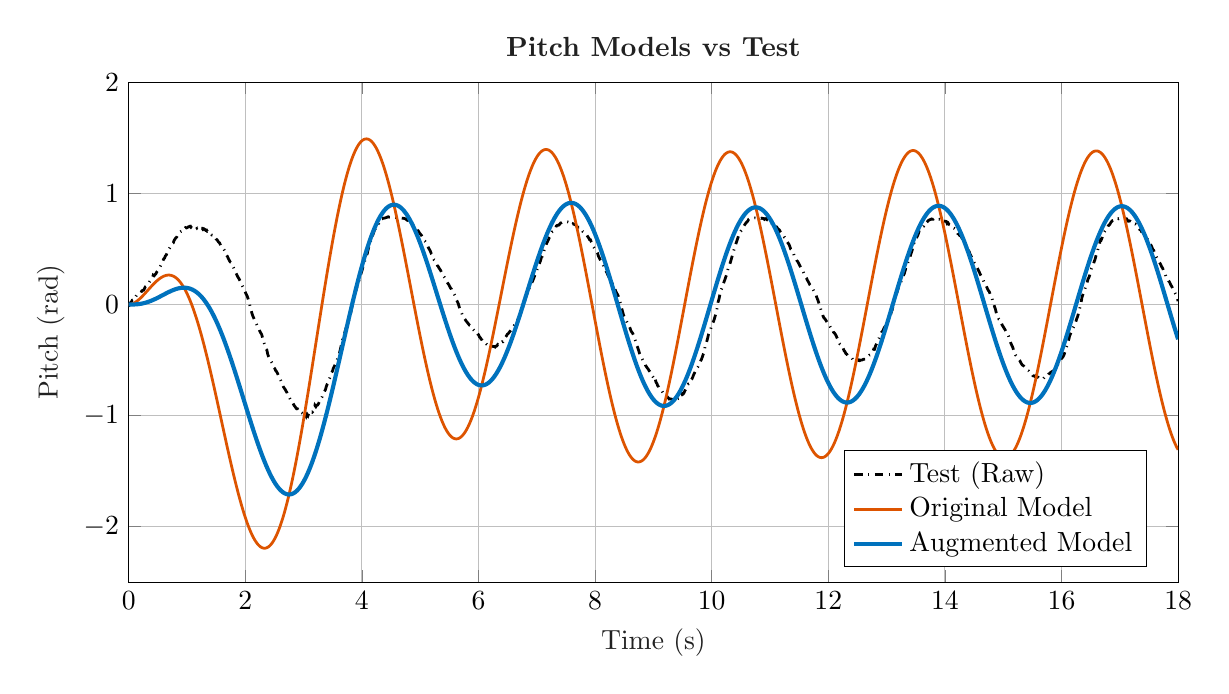
\begin{tikzpicture}

\begin{axis}[%
width=5.247in,
height=2.498in,
at={(0.88in,0.392in)},
scale only axis,
xmin=0,
xmax=18,
xlabel style={font=\color{mycolor3}},
xlabel={Time (s)},
ymin=-2.5,
ymax=2,
ylabel style={font=\color{mycolor3}},
ylabel={Pitch (rad)},
axis background/.style={fill=white},
title style={font=\bfseries\color{mycolor3}},
title={Pitch Models vs Test},
xmajorgrids,
ymajorgrids,
legend style={at={(0.97,0.03)}, anchor=south east, legend cell align=left, align=left}
]
\addplot [color=black, dashdotted, line width=1.0pt]
  table[row sep=crcr]{%
0	-0.0195601059887639\\
0.015	0.0074208779410081\\
0.03	0.0164145392509321\\
0.045	0.0225680969893011\\
0.06	0.0391353678233716\\
0.075	0.0419754713949266\\
0.09	0.0509691327048505\\
0.105	0.0727432600867717\\
0.12	0.0699031565152168\\
0.135	0.0839675093465895\\
0.15	0.0862395922038334\\
0.165	0.0902157372040103\\
0.18	0.0998720893472971\\
0.195	0.104984275776096\\
0.21	0.106972348276184\\
0.225	0.122876928276892\\
0.24	0.127137083634224\\
0.255	0.128557135420002\\
0.27	0.143041663634932\\
0.285	0.160366295421417\\
0.3	0.166046502564527\\
0.315	0.175134833993503\\
0.33	0.182519103279546\\
0.345	0.192459465779988\\
0.36	0.207512014709229\\
0.375	0.218020397923982\\
0.39	0.229096801853046\\
0.405	0.2370490918534\\
0.42	0.264331912615593\\
0.435	0.258651705472483\\
0.45	0.268341470598964\\
0.465	0.27602645673376\\
0.48	0.292398818499194\\
0.495	0.303759232785414\\
0.51	0.320465724382796\\
0.525	0.330489619341225\\
0.54	0.341515903795497\\
0.555	0.357554135728984\\
0.57	0.383950392452848\\
0.585	0.389964729427905\\
0.6	0.410680779008659\\
0.615	0.418699894975402\\
0.63	0.438602558630848\\
0.645	0.446904399840008\\
0.66	0.467003594346397\\
0.675	0.479237886654634\\
0.69	0.502395654238082\\
0.705	0.511134434458251\\
0.72	0.525116482810521\\
0.735	0.543467921272876\\
0.75	0.55089588446002\\
0.765	0.555265274570104\\
0.78	0.578423042153552\\
0.795	0.590657334461789\\
0.81	0.601499609021305\\
0.825	0.608315857593037\\
0.84	0.62762856187961\\
0.855	0.638231615213415\\
0.87	0.646562585689977\\
0.885	0.654136195214123\\
0.9	0.659437721881026\\
0.915	0.662845846166892\\
0.93	0.662088485214477\\
0.945	0.674206260453111\\
0.96	0.677993065215185\\
0.975	0.69276160378727\\
0.99	0.690110840453819\\
1.005	0.69276160378727\\
1.02	0.699199171882795\\
1.035	0.700713893787624\\
1.05	0.704879379025905\\
1.065	0.696548408549344\\
1.08	0.707530142359356\\
1.095	0.710938266645222\\
1.11	0.702985976644868\\
1.125	0.70412201807349\\
1.14	0.705636739978319\\
1.155	0.702607296168661\\
1.17	0.690489520930026\\
1.185	0.702228615692453\\
1.2	0.696169728073136\\
1.215	0.688974799025197\\
1.23	0.689353479501404\\
1.245	0.687460077120368\\
1.26	0.687460077120368\\
1.275	0.676099662834148\\
1.29	0.682158550453465\\
1.305	0.676478343310355\\
1.32	0.668147372833794\\
1.335	0.670798136167245\\
1.35	0.658301680452404\\
1.365	0.66019508283344\\
1.38	0.649970709975843\\
1.395	0.642775780927903\\
1.41	0.640882378546867\\
1.425	0.626871200927196\\
1.44	0.62762856187961\\
1.455	0.612860023307525\\
1.47	0.610966620926488\\
1.485	0.600363567592683\\
1.5	0.588909578417755\\
1.515	0.583666310285654\\
1.53	0.570995078966409\\
1.545	0.560508542702206\\
1.56	0.554391396548087\\
1.575	0.533418324019682\\
1.59	0.522931787755479\\
1.605	0.518562397645394\\
1.62	0.505454227315141\\
1.635	0.494093813028921\\
1.65	0.479237886654634\\
1.665	0.469625228412448\\
1.68	0.442535009729924\\
1.695	0.431611534454713\\
1.71	0.413019687832292\\
1.725	0.397983845394648\\
1.74	0.384284522284795\\
1.755	0.379272574805581\\
1.77	0.360561304216513\\
1.785	0.345525461778869\\
1.8	0.330155489509278\\
1.815	0.31144421892021\\
1.83	0.295071857154775\\
1.845	0.278365365557394\\
1.86	0.261658873960012\\
1.875	0.246137423282376\\
1.89	0.234777008996156\\
1.905	0.217736387566827\\
1.92	0.203251859351897\\
1.935	0.186211237922567\\
1.95	0.168602595778926\\
1.965	0.155254108992618\\
1.98	0.135657394348889\\
1.995	0.118332762562404\\
2.01	0.0987360479186751\\
2.025	0.084251519703745\\
2.04	0.0651696505626252\\
2.055	0.0396087184186308\\
2.07	0.0107343321078222\\
2.085	-0.0247669625366146\\
2.1	-0.0522212970616457\\
2.115	-0.0815690339677134\\
2.13	-0.104147263658346\\
2.145	-0.122478841256564\\
2.16	-0.140810418854782\\
2.175	-0.155010936712557\\
2.19	-0.173342514310775\\
2.205	-0.191674091908993\\
2.22	-0.204067271130324\\
2.235	-0.222140657494764\\
2.25	-0.242021382495649\\
2.265	-0.255705517885868\\
2.28	-0.268615079574754\\
2.295	-0.297725474363541\\
2.31	-0.320009363924972\\
2.325	-0.349284277662539\\
2.34	-0.368946533157919\\
2.355	-0.399969202939519\\
2.37	-0.409581861181705\\
2.385	-0.448906372172466\\
2.4	-0.469883812665944\\
2.415	-0.486326517553894\\
2.43	-0.497089015298734\\
2.445	-0.515026511540133\\
2.46	-0.527283800638423\\
2.475	-0.546417129962583\\
2.49	-0.568540041993642\\
2.505	-0.576312957031582\\
2.52	-0.593951495002291\\
2.535	-0.602920243122991\\
2.55	-0.617270240116111\\
2.565	-0.635352721800089\\
2.58	-0.648133187872086\\
2.595	-0.669433964658748\\
2.61	-0.686001235492818\\
2.625	-0.706828661684221\\
2.64	-0.722922581923033\\
2.655	-0.742803306923917\\
2.67	-0.754637071805396\\
2.685	-0.765524135496357\\
2.7	-0.78019800394939\\
2.715	-0.794398521807165\\
2.73	-0.816506091509761\\
2.745	-0.834177847066103\\
2.76	-0.842382590717262\\
2.775	-0.858160943892567\\
2.79	-0.864472285162689\\
2.805	-0.885299711354092\\
2.82	-0.891611052624214\\
2.835	-0.908020539926531\\
2.85	-0.917487551831714\\
2.865	-0.929479100244947\\
2.88	-0.939577246277142\\
2.895	-0.939577246277142\\
2.91	-0.954724465325435\\
2.925	-0.950306526436349\\
2.94	-0.964191477230618\\
2.955	-0.971765086754764\\
2.97	-0.976048823086156\\
2.985	-0.980782329038747\\
3	-1.00160975523015\\
3.015	-0.983622432610302\\
3.03	-0.99024934094393\\
3.045	-1.00728996237326\\
3.06	-0.988355938562894\\
3.075	-1.00066305403963\\
3.09	-0.977942225467192\\
3.105	-0.969240550246716\\
3.12	-0.96482261135763\\
3.135	-0.95914240421452\\
3.15	-0.968609416119703\\
3.165	-0.960404672468545\\
3.18	-0.951568794690374\\
3.195	-0.908651674053544\\
3.21	-0.920012088339763\\
3.225	-0.906758271672507\\
3.24	-0.905496003418482\\
3.255	-0.893504455005251\\
3.27	-0.875201565321897\\
3.285	-0.869521358178787\\
3.3	-0.84490712722531\\
3.315	-0.833546712939091\\
3.33	-0.808932481985615\\
3.345	-0.793925171211906\\
3.36	-0.78019800394939\\
3.375	-0.765524135496357\\
3.39	-0.737123099780807\\
3.405	-0.716295673589404\\
3.42	-0.704461908707926\\
3.435	-0.673220769420821\\
3.45	-0.659966952753565\\
3.465	-0.64055957834794\\
3.48	-0.611888991243691\\
3.495	-0.600229618686781\\
3.51	-0.573622332595372\\
3.525	-0.557478585978112\\
3.54	-0.542231714172923\\
3.555	-0.525789009284973\\
3.57	-0.504861930336673\\
3.585	-0.485728601012514\\
3.6	-0.462409855898694\\
3.615	-0.438419835908263\\
3.63	-0.403464715027587\\
3.645	-0.368946533157919\\
3.66	-0.332680595244218\\
3.675	-0.295540779308499\\
3.69	-0.27016422697742\\
3.705	-0.255705517885868\\
3.72	-0.22601352600143\\
3.735	-0.201485358792546\\
3.75	-0.177989956518774\\
3.765	-0.153203598076113\\
3.78	-0.13306468184145\\
3.795	-0.109827470801455\\
3.81	-0.0716286714672711\\
3.825	-0.0304471696797245\\
3.84	0.0135744356793771\\
3.855	0.0575960410384787\\
3.87	0.0816954264893455\\
3.885	0.11038047256205\\
3.9	0.129977187205779\\
3.915	0.15894624363564\\
3.93	0.186211237922567\\
3.945	0.208364045780695\\
3.96	0.231936905424601\\
3.975	0.259654094968326\\
3.99	0.288055130683875\\
4.005	0.311110089088262\\
4.02	0.345859591610817\\
4.035	0.36523912186378\\
4.05	0.39497667690712\\
4.065	0.413687947496187\\
4.08	0.442098070718915\\
4.095	0.465255838302364\\
4.11	0.503706471271107\\
4.125	0.532107506986656\\
4.14	0.552643640504054\\
4.155	0.583229371274645\\
4.17	0.622327035212708\\
4.185	0.623841757117537\\
4.2	0.646183905213769\\
4.215	0.668904733786209\\
4.23	0.68291591140588\\
4.245	0.690110840453819\\
4.26	0.717375834740746\\
4.275	0.729872290455588\\
4.29	0.731765692836625\\
4.305	0.751835758075613\\
4.32	0.761681450457003\\
4.335	0.772284503790808\\
4.35	0.773428853382733\\
4.365	0.777579773987313\\
4.38	0.778235182503826\\
4.395	0.779109060525843\\
4.41	0.782495337861158\\
4.425	0.784352328657944\\
4.44	0.789486362037293\\
4.455	0.790032535801054\\
4.47	0.786755493218491\\
4.485	0.786100084701978\\
4.5	0.788066310251516\\
4.515	0.785881615196474\\
4.53	0.786755493218491\\
4.545	0.784461563410696\\
4.56	0.784789267668953\\
4.575	0.783806154894183\\
4.59	0.783587685388679\\
4.605	0.784243093905192\\
4.62	0.784243093905192\\
4.635	0.782713807366662\\
4.65	0.779109060525843\\
4.665	0.778016712998321\\
4.68	0.778562886762082\\
4.695	0.777798243492817\\
4.71	0.777579773987313\\
4.725	0.775504313685023\\
4.74	0.772882679618972\\
4.755	0.771905823314601\\
4.77	0.760924089504589\\
4.785	0.75789464569493\\
4.8	0.755243882361479\\
4.815	0.743126107122844\\
4.83	0.73668853902732\\
4.845	0.730629651408003\\
4.86	0.728357568550759\\
4.875	0.715103751883502\\
4.89	0.703743337597283\\
4.905	0.701471254740039\\
4.92	0.695791047596929\\
4.935	0.686324035691746\\
4.95	0.670040775214831\\
4.965	0.664739248547928\\
4.98	0.651106751404465\\
4.995	0.63898897616583\\
5.01	0.630658005689269\\
5.025	0.620433632831671\\
5.04	0.607179816164415\\
5.055	0.592842029516831\\
5.07	0.574053652043468\\
5.085	0.567936505889349\\
5.1	0.557449969625146\\
5.115	0.538661592151783\\
5.13	0.524242604788504\\
5.145	0.507638922370183\\
5.16	0.49453075203993\\
5.175	0.479237886654634\\
5.19	0.458264814126228\\
5.205	0.448652155884042\\
5.22	0.422041193294878\\
5.235	0.405000571865549\\
5.25	0.399654494554387\\
5.265	0.382613873125057\\
5.28	0.368246290351309\\
5.295	0.350203279426136\\
5.31	0.341850033627445\\
5.325	0.326814191189801\\
5.34	0.316122036567477\\
5.355	0.302422713457624\\
5.37	0.285382092028294\\
5.385	0.268675600430912\\
5.4	0.252303238665478\\
5.415	0.24528539221091\\
5.43	0.229948832924513\\
5.445	0.214328263280961\\
5.46	0.201831807566119\\
5.475	0.189619362208433\\
5.49	0.17911097899368\\
5.505	0.163206398992972\\
5.52	0.148437860420886\\
5.535	0.139065518634755\\
5.55	0.11861677291956\\
5.565	0.106120317204718\\
5.58	0.0956119339899647\\
5.595	0.0828314679179675\\
5.61	0.0651696505626252\\
5.625	0.0386620172281124\\
5.64	0.0235147981798194\\
5.655	0.00458077436945316\\
5.67	-0.0233469107508371\\
5.685	-0.04417433694224\\
5.7	-0.0650017631336429\\
5.715	-0.0825157351582317\\
5.73	-0.106470984762345\\
5.745	-0.116024060412121\\
5.76	-0.127900857165896\\
5.775	-0.137970315283227\\
5.79	-0.150879876972113\\
5.805	-0.158625613985445\\
5.82	-0.169727837037887\\
5.835	-0.179280912687662\\
5.85	-0.18754303216855\\
5.865	-0.190641326973882\\
5.88	-0.210522051974767\\
5.895	-0.219042362689431\\
5.91	-0.226271717235208\\
5.925	-0.234275645482317\\
5.94	-0.243828721132093\\
5.955	-0.240472235092982\\
5.97	-0.25544732665209\\
5.985	-0.265516784769421\\
6	-0.271455183146309\\
6.015	-0.289860572165389\\
6.03	-0.29816241337455\\
6.045	-0.312581400737829\\
6.06	-0.318698546891947\\
6.075	-0.332243656233209\\
6.09	-0.335739168321277\\
6.105	-0.347099582607497\\
6.12	-0.346662643596488\\
6.135	-0.355401423816657\\
6.15	-0.361518569970775\\
6.165	-0.368509594146911\\
6.18	-0.364140204036826\\
6.195	-0.369383472168928\\
6.21	-0.378996130411113\\
6.225	-0.375063679312037\\
6.24	-0.375063679312037\\
6.255	-0.378122252389097\\
6.27	-0.377685313378088\\
6.285	-0.382928581510189\\
6.3	-0.374626740301029\\
6.315	-0.372005106234978\\
6.33	-0.360644691948758\\
6.345	-0.367198777113885\\
6.36	-0.356275301838674\\
6.375	-0.349721216673547\\
6.39	-0.34316713150842\\
6.405	-0.33486529029926\\
6.42	-0.335302229310268\\
6.435	-0.319135485902956\\
6.45	-0.30384262051766\\
6.465	-0.292919145242448\\
6.48	-0.281558730956229\\
6.495	-0.267324123405865\\
6.51	-0.261385725028978\\
6.525	-0.251058075677869\\
6.54	-0.241763191261871\\
6.555	-0.230144585741873\\
6.57	-0.218525980221876\\
6.585	-0.206390992234323\\
6.6	-0.201227167558769\\
6.615	-0.186252075999661\\
6.63	-0.176440809116107\\
6.645	-0.166113159764999\\
6.66	-0.151138068205891\\
6.675	-0.135130211711672\\
6.69	-0.124286179893008\\
6.705	-0.101823542554346\\
6.72	-0.0867758905155641\\
6.735	-0.0678418667051979\\
6.75	-0.0484344922995724\\
6.765	-0.00819969170254409\\
6.78	0.0301417065134476\\
6.795	0.0381886666328533\\
6.81	0.0780032918463241\\
6.825	0.0893637061325438\\
6.84	0.105268286133251\\
6.855	0.141621611849155\\
6.87	0.146733798277953\\
6.885	0.166898533635993\\
6.9	0.181099051493768\\
6.915	0.197287641851631\\
6.93	0.21376024256665\\
6.945	0.234208988281845\\
6.96	0.254976277321059\\
6.975	0.275358197069865\\
6.99	0.293401207995037\\
7.005	0.316456166399424\\
7.02	0.331157879005121\\
7.035	0.36089543404846\\
7.05	0.375597146654157\\
7.065	0.397983845394648\\
7.08	0.428116022366645\\
7.095	0.434670107531772\\
7.11	0.461760326214296\\
7.125	0.48885054489682\\
7.14	0.512445251491276\\
7.155	0.525990360832538\\
7.17	0.554391396548087\\
7.185	0.567936505889349\\
7.2	0.585414066329687\\
7.215	0.603393011402342\\
7.23	0.614374745212354\\
7.245	0.637474254261001\\
7.26	0.653378834261709\\
7.275	0.657165639023782\\
7.29	0.669283414262416\\
7.305	0.671934177595867\\
7.32	0.685566674739331\\
7.335	0.707908822835563\\
7.35	0.713210349502466\\
7.365	0.713589029978673\\
7.38	0.715861112835917\\
7.395	0.725706805217307\\
7.41	0.734795136646283\\
7.425	0.737445899979735\\
7.44	0.741990065694222\\
7.455	0.741232704741808\\
7.47	0.739717982836979\\
7.485	0.743126107122844\\
7.5	0.745776870456296\\
7.515	0.746155550932503\\
7.53	0.744262148551466\\
7.545	0.741611385218015\\
7.56	0.738581941408357\\
7.575	0.737824580455942\\
7.59	0.727600207598344\\
7.605	0.719269237121783\\
7.62	0.727600207598344\\
7.635	0.722298680931441\\
7.65	0.721920000455234\\
7.665	0.716239793312124\\
7.68	0.708666183787978\\
7.695	0.695033686644514\\
7.71	0.696927089025551\\
7.725	0.697305769501758\\
7.74	0.678750426167599\\
7.755	0.673448899500697\\
7.77	0.672312858072075\\
7.785	0.659437721881026\\
7.8	0.654136195214123\\
7.815	0.645805224737562\\
7.83	0.644290502832733\\
7.845	0.631036686165476\\
7.86	0.62346307664133\\
7.875	0.610587940450281\\
7.89	0.599606206640268\\
7.905	0.584977127318679\\
7.92	0.583229371274645\\
7.935	0.563130176768256\\
7.95	0.550458945449011\\
7.965	0.52555342182153\\
7.98	0.513756068524301\\
7.995	0.499774020172031\\
8.01	0.487102788852786\\
8.025	0.4774901306106\\
8.04	0.46612971632438\\
8.055	0.439039497641856\\
8.07	0.422041193294878\\
8.085	0.405668831529444\\
8.1	0.387959950436219\\
8.115	0.378938444973633\\
8.13	0.365907381527675\\
8.145	0.34819850043445\\
8.16	0.326814191189801\\
8.175	0.319463334886953\\
8.19	0.297410765978409\\
8.205	0.284045572700503\\
8.22	0.264331912615593\\
8.235	0.249296070177949\\
8.25	0.235061019353312\\
8.265	0.214328263280961\\
8.28	0.206375973280607\\
8.295	0.191607434708521\\
8.31	0.175702854707814\\
8.325	0.15894624363564\\
8.34	0.141621611849155\\
8.355	0.117480731490938\\
8.37	0.102712192918852\\
8.385	0.0902157372040103\\
8.4	0.0722699094915126\\
8.415	0.0471823279427773\\
8.43	0.0197279934177462\\
8.445	-0.0167200024172089\\
8.46	-0.0418075839659442\\
8.475	-0.071155320872012\\
8.49	-0.0995563565875613\\
8.505	-0.11266757437301\\
8.52	-0.129191813334785\\
8.535	-0.147523390933003\\
8.55	-0.162756673725888\\
8.565	-0.177989956518774\\
8.58	-0.190124944506327\\
8.595	-0.207423757169434\\
8.61	-0.229111820806763\\
8.625	-0.245894251002314\\
8.64	-0.25544732665209\\
8.655	-0.271196991912531\\
8.67	-0.288549755132364\\
8.685	-0.316076912825896\\
8.7	-0.337486924365311\\
8.715	-0.370694289201953\\
8.73	-0.386424093598257\\
8.745	-0.410018800192714\\
8.76	-0.437982896897254\\
8.775	-0.454636940860755\\
8.79	-0.473172353643534\\
8.805	-0.486625475824584\\
8.82	-0.501872347629774\\
8.835	-0.516820261164273\\
8.85	-0.526984842367733\\
8.865	-0.548210879586722\\
8.88	-0.559272335602252\\
8.895	-0.571529624700542\\
8.91	-0.580797331091932\\
8.925	-0.595745244626431\\
8.94	-0.604415034476441\\
8.955	-0.617270240116111\\
8.97	-0.628725813466461\\
8.985	-0.646239785491049\\
9	-0.656653498586751\\
9.015	-0.680321028349709\\
9.03	-0.668013912872971\\
9.045	-0.700201753350593\\
9.06	-0.712035518232072\\
9.075	-0.733336295018734\\
9.09	-0.741856605733399\\
9.105	-0.756530474186433\\
9.12	-0.764577434305838\\
9.135	-0.774044446211021\\
9.15	-0.781618055735168\\
9.165	-0.796765274783461\\
9.18	-0.802621140715493\\
9.195	-0.808301347858603\\
9.21	-0.812719286747688\\
9.225	-0.817768359763786\\
9.24	-0.832915578812079\\
9.255	-0.841120322463237\\
9.27	-0.851218468495433\\
9.285	-0.849325066114396\\
9.3	-0.85058733436842\\
9.315	-0.854374139130494\\
9.33	-0.854374139130494\\
9.345	-0.853743005003481\\
9.36	-0.858160943892567\\
9.375	-0.846800529606347\\
9.39	-0.84490712722531\\
9.405	-0.853111870876469\\
9.42	-0.848062797860372\\
9.435	-0.84490712722531\\
9.45	-0.82471083516092\\
9.465	-0.818399493890798\\
9.48	-0.799465470080432\\
9.495	-0.811457018493663\\
9.51	-0.806407945477566\\
9.525	-0.794871872402424\\
9.54	-0.775937848592058\\
9.555	-0.762684031924802\\
9.57	-0.753690370614878\\
9.585	-0.738543151566585\\
9.6	-0.716295673589404\\
9.615	-0.716295673589404\\
9.63	-0.700675103945852\\
9.645	-0.678900976563931\\
9.66	-0.670380665849266\\
9.675	-0.653340044419937\\
9.69	-0.632512618228534\\
9.705	-0.616971281845421\\
9.72	-0.602322326581611\\
9.735	-0.590961912295391\\
9.75	-0.566148375828122\\
9.765	-0.558973377331562\\
9.78	-0.538644214924643\\
9.795	-0.528479633721183\\
9.81	-0.509047346126333\\
9.825	-0.492006724697004\\
9.84	-0.471079645748704\\
9.855	-0.446721677117423\\
9.87	-0.430117994699102\\
9.885	-0.382928581510189\\
9.9	-0.362392447992792\\
9.915	-0.332243656233209\\
9.93	-0.303405681506651\\
9.945	-0.268615079574754\\
9.96	-0.250541693210313\\
9.975	-0.233242880547206\\
9.99	-0.206907374701879\\
10.005	-0.175149852947219\\
10.02	-0.164305821128555\\
10.035	-0.147007008465447\\
10.05	-0.12067150262012\\
10.065	-0.0938761494444515\\
10.08	-0.0664218149194204\\
10.095	-0.0238202613460963\\
10.11	0.0230414475845603\\
10.125	0.0500224315143322\\
10.14	0.0893637061325438\\
10.155	0.127989114705691\\
10.17	0.141337601491999\\
10.185	0.156958171135551\\
10.2	0.186495248279722\\
10.215	0.208932066495006\\
10.23	0.23136888471029\\
10.245	0.253639757993268\\
10.26	0.27602645673376\\
10.275	0.311778348752157\\
10.29	0.335167436988492\\
10.305	0.355883486569246\\
10.32	0.379272574805581\\
10.335	0.407005350857235\\
10.35	0.434670107531772\\
10.365	0.46044950918127\\
10.38	0.490598300940854\\
10.395	0.515066885557327\\
10.41	0.538224653140775\\
10.425	0.564004054790273\\
10.44	0.586724883362713\\
10.455	0.610209259974073\\
10.47	0.632551408070306\\
10.485	0.643911822356525\\
10.5	0.66019508283344\\
10.515	0.667011331405172\\
10.53	0.68859611854899\\
10.545	0.700713893787624\\
10.56	0.713210349502466\\
10.575	0.726464166169722\\
10.59	0.735931178074905\\
10.605	0.744262148551466\\
10.62	0.753350479980442\\
10.635	0.768876379504942\\
10.65	0.773647322888237\\
10.665	0.772991914371724\\
10.68	0.773647322888237\\
10.695	0.775067374674014\\
10.71	0.776596661212544\\
10.725	0.778672121514834\\
10.74	0.780092173300612\\
10.755	0.778562886762082\\
10.77	0.778016712998321\\
10.785	0.777142834976305\\
10.8	0.778016712998321\\
10.815	0.776815130718048\\
10.83	0.778016712998321\\
10.845	0.775285844179519\\
10.86	0.778016712998321\\
10.875	0.775941252696031\\
10.89	0.774630435663006\\
10.905	0.767361657600113\\
10.92	0.773210383877229\\
10.935	0.774193496651998\\
10.95	0.762817491885625\\
10.965	0.760924089504589\\
10.98	0.756758604266308\\
10.995	0.746155550932503\\
11.01	0.747670272837332\\
11.025	0.736309858551113\\
11.04	0.723434722360063\\
11.055	0.727221527122137\\
11.07	0.710938266645222\\
11.085	0.717754515216954\\
11.1	0.702228615692453\\
11.115	0.69844181093038\\
11.13	0.683673272358294\\
11.145	0.678371745691392\\
11.16	0.671934177595867\\
11.175	0.657165639023782\\
11.19	0.646562585689977\\
11.205	0.637852934737208\\
11.22	0.633687449498928\\
11.235	0.621569674260293\\
11.25	0.604529052830964\\
11.265	0.599606206640268\\
11.28	0.582355493252628\\
11.295	0.563567115779265\\
11.31	0.553080579515062\\
11.325	0.542594043250859\\
11.34	0.522931787755479\\
11.355	0.499337081161023\\
11.37	0.492782995995896\\
11.385	0.472246862478499\\
11.4	0.465255838302364\\
11.415	0.439039497641856\\
11.43	0.42037054413514\\
11.445	0.414022077328135\\
11.46	0.39631319623491\\
11.475	0.387291690772324\\
11.49	0.371921718502732\\
11.505	0.356551746233141\\
11.52	0.34251829329134\\
11.535	0.329153100013435\\
11.55	0.311110089088262\\
11.565	0.300417934465938\\
11.58	0.282709053372713\\
11.595	0.272351028582336\\
11.61	0.248693516496775\\
11.625	0.238753153996333\\
11.64	0.220008470424071\\
11.655	0.207228004352073\\
11.67	0.191607434708521\\
11.685	0.177406916850747\\
11.7	0.168886606136082\\
11.715	0.154118067563996\\
11.73	0.142757653277777\\
11.745	0.128841145777157\\
11.76	0.113504586490761\\
11.775	0.0950439132756537\\
11.79	0.083683498989434\\
11.805	0.061382845800552\\
11.82	0.0410287702044082\\
11.835	0.0173612404414504\\
11.85	-0.0115131458693582\\
11.865	-0.0299738190844653\\
11.88	-0.0597949065857922\\
11.895	-0.0758888268246035\\
11.91	-0.104405454892123\\
11.925	-0.121446076321453\\
11.94	-0.127126283464563\\
11.955	-0.139261271452116\\
11.97	-0.151654450673446\\
11.985	-0.162756673725888\\
12	-0.179022721453885\\
12.015	-0.182121016259217\\
12.03	-0.198128872753436\\
12.045	-0.212329390611211\\
12.06	-0.228079055871652\\
12.075	-0.22601352600143\\
12.09	-0.250283501976536\\
12.105	-0.256738282820979\\
12.12	-0.267324123405865\\
12.135	-0.281558730956229\\
12.15	-0.300784047440601\\
12.165	-0.314766095792871\\
12.18	-0.331806717222201\\
12.195	-0.353216728761615\\
12.21	-0.358023057882708\\
12.225	-0.373315923268004\\
12.24	-0.394288995796409\\
12.255	-0.394725934807418\\
12.27	-0.415262068324815\\
12.285	-0.423563909533975\\
12.3	-0.440604530963305\\
12.315	-0.446284738106415\\
12.33	-0.457626523567655\\
12.345	-0.462409855898694\\
12.36	-0.468687979583184\\
12.375	-0.474069228455604\\
12.39	-0.479749435598714\\
12.405	-0.482440060034924\\
12.42	-0.495295265674594\\
12.435	-0.491109849884934\\
12.45	-0.493501516050454\\
12.465	-0.496192140486664\\
12.48	-0.497985890110804\\
12.495	-0.504562972065983\\
12.51	-0.504562972065983\\
12.525	-0.498583806652184\\
12.54	-0.505160888607363\\
12.555	-0.500676514547014\\
12.57	-0.499480681464254\\
12.585	-0.498583806652184\\
12.6	-0.493501516050454\\
12.615	-0.492305682967694\\
12.63	-0.492006724697004\\
12.645	-0.487821308907344\\
12.66	-0.480945268681474\\
12.675	-0.471378604019394\\
12.69	-0.465100480334904\\
12.705	-0.456729648755585\\
12.72	-0.454337982590065\\
12.735	-0.446284738106415\\
12.75	-0.434924323820195\\
12.765	-0.420942275467925\\
12.78	-0.400406141950528\\
12.795	-0.401280019972544\\
12.81	-0.372005106234978\\
12.825	-0.355838362827666\\
12.84	-0.338360802387327\\
12.855	-0.31520303480388\\
12.87	-0.304279559528668\\
12.885	-0.280247913923203\\
12.9	-0.269131462042309\\
12.915	-0.248992545807647\\
12.93	-0.242279573729426\\
12.945	-0.22601352600143\\
12.96	-0.206907374701879\\
12.975	-0.197096107818325\\
12.99	-0.182121016259217\\
13.005	-0.169986028271664\\
13.02	-0.149072538335669\\
13.035	-0.134097446776561\\
13.05	-0.121962458789008\\
13.065	-0.102598116255679\\
13.08	-0.0664218149194204\\
13.095	-0.0498545440853499\\
13.11	-0.0124598470598765\\
13.125	0.0197279934177462\\
13.14	0.0599627940147745\\
13.155	0.080843395417879\\
13.17	0.0995880789901416\\
13.185	0.121456876491115\\
13.2	0.149005881135197\\
13.215	0.168034575064615\\
13.23	0.188767331136966\\
13.245	0.200695766137497\\
13.26	0.223984615424248\\
13.275	0.239037164353489\\
13.29	0.262661263455854\\
13.305	0.280704274381027\\
13.32	0.309773569760472\\
13.335	0.337506345812126\\
13.35	0.357888265560932\\
13.365	0.379272574805581\\
13.38	0.397649715562701\\
13.395	0.414022077328135\\
13.41	0.446030521817992\\
13.425	0.467440533357406\\
13.44	0.491035239951862\\
13.455	0.546526494349935\\
13.47	0.553080579515062\\
13.485	0.586724883362713\\
13.5	0.592842029516831\\
13.515	0.602635650449927\\
13.53	0.619297591403049\\
13.545	0.63898897616583\\
13.56	0.666632650928965\\
13.575	0.667768692357587\\
13.59	0.685187994263124\\
13.605	0.690489520930026\\
13.62	0.701471254740039\\
13.635	0.704879379025905\\
13.65	0.724949444264893\\
13.665	0.740475343789393\\
13.68	0.735931178074905\\
13.695	0.743883468075259\\
13.71	0.754107840932857\\
13.725	0.760166728552174\\
13.74	0.76357485283804\\
13.755	0.766225616171491\\
13.77	0.770769781885979\\
13.785	0.767740338076321\\
13.8	0.768497699028735\\
13.815	0.774630435663006\\
13.83	0.771905823314601\\
13.845	0.767740338076321\\
13.86	0.773210383877229\\
13.875	0.770012420933564\\
13.89	0.766225616171491\\
13.905	0.767361657600113\\
13.92	0.762817491885625\\
13.935	0.767740338076321\\
13.95	0.764332213790455\\
13.965	0.750321036170783\\
13.98	0.75221443855182\\
13.995	0.751078397123198\\
14.01	0.750321036170783\\
14.025	0.74804895331354\\
14.04	0.728357568550759\\
14.055	0.734037775693869\\
14.07	0.721541319979027\\
14.085	0.718511876169368\\
14.1	0.718511876169368\\
14.115	0.711695627597636\\
14.13	0.695412367120722\\
14.145	0.689732159977612\\
14.16	0.686324035691746\\
14.175	0.680265148072428\\
14.19	0.662467165690684\\
14.205	0.65602959759516\\
14.22	0.63898897616583\\
14.235	0.636338212832379\\
14.25	0.623084396165123\\
14.265	0.618918910926842\\
14.28	0.613238703783732\\
14.295	0.595026724571873\\
14.31	0.573616713032459\\
14.325	0.567499566878341\\
14.34	0.55919772566918\\
14.355	0.543030982261868\\
14.37	0.52249484874447\\
14.385	0.508075861381192\\
14.4	0.48885054489682\\
14.415	0.478800947643625\\
14.43	0.456080119071186\\
14.445	0.439039497641856\\
14.46	0.424183571267569\\
14.475	0.403329922705811\\
14.49	0.385955171444533\\
14.505	0.375931276486104\\
14.52	0.36657564119157\\
14.535	0.351873928585874\\
14.55	0.334499177324597\\
14.565	0.319129205055006\\
14.58	0.302088583625676\\
14.595	0.286050351692189\\
14.61	0.268007340767017\\
14.625	0.256312796648849\\
14.64	0.236197060781934\\
14.655	0.223984615424248\\
14.67	0.203535869709052\\
14.685	0.193311496851454\\
14.7	0.179963010065146\\
14.715	0.160934316135728\\
14.73	0.141621611849155\\
14.745	0.126569062919913\\
14.76	0.116912710776627\\
14.775	0.0947599029184982\\
14.79	0.08141141613219\\
14.805	0.0632762481815886\\
14.82	0.0320351088944842\\
14.835	0.0093142803220447\\
14.85	-0.0181400542029864\\
14.865	-0.0389674803943893\\
14.88	-0.0716286714672711\\
14.895	-0.100790777619235\\
14.91	-0.112151191905455\\
14.925	-0.131257343205006\\
14.94	-0.133839255542784\\
14.955	-0.156043701647668\\
14.97	-0.169211454570331\\
14.985	-0.187801223402327\\
15	-0.199419828922325\\
15.015	-0.212587581844988\\
15.03	-0.225497143533875\\
15.045	-0.240472235092982\\
15.06	-0.258287430223645\\
15.075	-0.267065932172088\\
15.09	-0.283306487000263\\
15.105	-0.311707522715812\\
15.12	-0.335302229310268\\
15.135	-0.352779789750606\\
15.15	-0.370694289201953\\
15.165	-0.387297971620274\\
15.18	-0.415262068324815\\
15.195	-0.429681055688094\\
15.21	-0.453740066048685\\
15.225	-0.463605688981454\\
15.24	-0.480347352140094\\
15.255	-0.487522350636654\\
15.27	-0.497985890110804\\
15.285	-0.506356721690123\\
15.3	-0.521304635224623\\
15.315	-0.535056715676363\\
15.33	-0.546118171691892\\
15.345	-0.550004629210862\\
15.36	-0.558076502519492\\
15.375	-0.566746292369502\\
15.39	-0.575117123948822\\
15.405	-0.587673371317802\\
15.42	-0.593652536731601\\
15.435	-0.597538994250571\\
15.45	-0.606806700641961\\
15.465	-0.612486907785071\\
15.48	-0.614280657409211\\
15.495	-0.628252462871202\\
15.51	-0.642452980728976\\
15.525	-0.642452980728976\\
15.54	-0.647659837276827\\
15.555	-0.642926331324235\\
15.57	-0.658546900967788\\
15.585	-0.654760096205714\\
15.6	-0.654286745610455\\
15.615	-0.664227108110897\\
15.63	-0.666120510491934\\
15.645	-0.661387004539343\\
15.66	-0.663753757515638\\
15.675	-0.663280406920379\\
15.69	-0.666593861087193\\
15.705	-0.656653498586751\\
15.72	-0.649079889062604\\
15.735	-0.643399681919495\\
15.75	-0.646239785491049\\
15.765	-0.636772773585866\\
15.78	-0.625412359299647\\
15.795	-0.622352530717841\\
15.81	-0.613084824326451\\
15.825	-0.607703575454031\\
15.84	-0.603518159664371\\
15.855	-0.601425451769541\\
15.87	-0.591260870566081\\
15.885	-0.580797331091932\\
15.9	-0.560169210414322\\
15.915	-0.554489003271212\\
15.93	-0.545819213421202\\
15.945	-0.535056715676363\\
15.96	-0.529376508533253\\
15.975	-0.509944220938403\\
15.99	-0.496192140486664\\
16.005	-0.480646310410784\\
16.02	-0.475265061538364\\
16.035	-0.461512981086624\\
16.05	-0.442352287007339\\
16.065	-0.41395125129179\\
16.08	-0.392104300741367\\
16.095	-0.370257350190944\\
16.11	-0.340982436453378\\
16.125	-0.313892217770854\\
16.14	-0.281558730956229\\
16.155	-0.262418489964089\\
16.17	-0.245894251002314\\
16.185	-0.225497143533875\\
16.2	-0.209747478273434\\
16.215	-0.195805151649437\\
16.23	-0.171018793206775\\
16.245	-0.156818275349001\\
16.26	-0.128417239633451\\
16.275	-0.110085662035233\\
16.29	-0.0810956833724542\\
16.305	-0.0583748548000147\\
16.32	-0.0162466518219498\\
16.335	0.013101085084118\\
16.35	0.0642229493721069\\
16.365	0.0870916232752999\\
16.38	0.108392400061962\\
16.395	0.126853073277069\\
16.41	0.153834057206841\\
16.425	0.170590668279015\\
16.44	0.200411755780342\\
16.455	0.230516853638824\\
16.47	0.24272929899651\\
16.485	0.266336691607278\\
16.5	0.293735337826985\\
16.515	0.326480061357854\\
16.53	0.338508735307969\\
16.545	0.35955891472067\\
16.56	0.385286911780638\\
16.575	0.407005350857235\\
16.59	0.437728680608831\\
16.605	0.460012570170262\\
16.62	0.48885054489682\\
16.635	0.519436275667411\\
16.65	0.5395354701738\\
16.665	0.584540188307671\\
16.68	0.581044676219603\\
16.695	0.60074224806889\\
16.71	0.628007242355818\\
16.725	0.642775780927903\\
16.74	0.657165639023782\\
16.755	0.668147372833794\\
16.77	0.687460077120368\\
16.785	0.689353479501404\\
16.8	0.707151461883149\\
16.815	0.716239793312124\\
16.83	0.722298680931441\\
16.845	0.738581941408357\\
16.86	0.74804895331354\\
16.875	0.756001243313893\\
16.89	0.759409367599759\\
16.905	0.771148462362186\\
16.92	0.768119018552528\\
16.935	0.773319618629981\\
16.95	0.77430273140475\\
16.965	0.774521200910254\\
16.98	0.772284503790808\\
16.995	0.776815130718048\\
17.01	0.775067374674014\\
17.025	0.774084261899245\\
17.04	0.770769781885979\\
17.055	0.773756557640989\\
17.07	0.774739670415758\\
17.085	0.774630435663006\\
17.1	0.772284503790808\\
17.115	0.772882679618972\\
17.13	0.759788048075967\\
17.145	0.750699716646991\\
17.16	0.754486521409064\\
17.175	0.751835758075613\\
17.19	0.74653423140871\\
17.205	0.737067219503527\\
17.22	0.732523053789039\\
17.235	0.732901734265247\\
17.25	0.723813402836271\\
17.265	0.724949444264893\\
17.28	0.716997154264539\\
17.295	0.707530142359356\\
17.31	0.696548408549344\\
17.325	0.693140284263478\\
17.34	0.676857023786563\\
17.355	0.677614384738977\\
17.37	0.659059041404818\\
17.385	0.661331124262062\\
17.4	0.646941266166184\\
17.415	0.638610295689623\\
17.43	0.62346307664133\\
17.445	0.618161549974427\\
17.46	0.597211419626916\\
17.475	0.58759876138473\\
17.49	0.575364469076493\\
17.505	0.560071603691197\\
17.52	0.543904860283885\\
17.535	0.534292202041699\\
17.55	0.517688519623378\\
17.565	0.495404630061947\\
17.58	0.489724422918837\\
17.595	0.46918828940144\\
17.61	0.45214766797211\\
17.625	0.42942683939967\\
17.64	0.416695115983716\\
17.655	0.405000571865549\\
17.67	0.386289301276481\\
17.685	0.374594757158314\\
17.7	0.362231953376251\\
17.715	0.342852423123288\\
17.73	0.332160268500963\\
17.745	0.313783127743843\\
17.76	0.292064688667247\\
17.775	0.28170666387687\\
17.79	0.254976277321059\\
17.805	0.244717371496599\\
17.82	0.231936905424601\\
17.835	0.213192221852339\\
17.85	0.204387900780519\\
17.865	0.188199310422655\\
17.88	0.171726709707637\\
17.895	0.15894624363564\\
17.91	0.143041663634932\\
17.925	0.123444948991203\\
17.94	0.112368545062139\\
17.955	0.0973159961328976\\
17.97	0.084251519703745\\
17.985	0.0575960410384787\\
18	0.0306150571087068\\
};
\addlegendentry{Test (Raw)}

\addplot [color=mycolor1, line width=1.0pt]
  table[row sep=crcr]{%
0	0\\
0.015	0.000395410560298629\\
0.03	0.00156157507277703\\
0.045	0.00346227679358755\\
0.06	0.00606100084311244\\
0.075	0.00932096946067302\\
0.09	0.0132051773774006\\
0.105	0.0176764272767039\\
0.12	0.0226973653116957\\
0.135	0.0282305166488973\\
0.15	0.0342383210075231\\
0.165	0.0406831681636562\\
0.18	0.0475274333886643\\
0.195	0.0547335127912708\\
0.21	0.0622638585327848\\
0.225	0.0700810138851153\\
0.24	0.0781476481013405\\
0.255	0.086426591068773\\
0.27	0.0948808677146643\\
0.285	0.103473732134917\\
0.3	0.112168701416421\\
0.315	0.12092958912392\\
0.33	0.1297205384226\\
0.345	0.138506054807942\\
0.36	0.147251038414716\\
0.375	0.155920815877398\\
0.39	0.164481171714656\\
0.405	0.172898379211042\\
0.42	0.181139230769405\\
0.435	0.189171067708082\\
0.45	0.196961809477385\\
0.465	0.204479982270427\\
0.48	0.211694747003905\\
0.495	0.218575926644971\\
0.51	0.225094032860963\\
0.525	0.231220291969337\\
0.54	0.236926670165791\\
0.555	0.242185898009198\\
0.57	0.246971494142666\\
0.585	0.251257788230683\\
0.6	0.255019943093042\\
0.615	0.258233976016956\\
0.63	0.260876779229475\\
0.645	0.26292613951313\\
0.66	0.264360756948429\\
0.675	0.265160262767675\\
0.69	0.265305236305305\\
0.705	0.264777221030826\\
0.72	0.263558739651184\\
0.735	0.261633308270282\\
0.75	0.258985449594169\\
0.765	0.255600705171297\\
0.78	0.251465646658104\\
0.795	0.246567886101042\\
0.81	0.240896085227056\\
0.825	0.234439963735402\\
0.84	0.227190306584591\\
0.855	0.219138970269125\\
0.87	0.21027888808163\\
0.885	0.200604074356842\\
0.9	0.190109627694874\\
0.915	0.178791733162047\\
0.93	0.166647663468517\\
0.945	0.153675779122827\\
0.96	0.139875527564432\\
0.975	0.125247441276153\\
0.99	0.109793134879425\\
1.005	0.0935153012161121\\
1.02	0.0764177064215795\\
1.035	0.0585051839945768\\
1.05	0.0397836278704249\\
1.065	0.0202599845048526\\
1.08	-5.77560232731863e-05\\
1.095	-0.0211605698812093\\
1.11	-0.043038410313612\\
1.125	-0.0656802194249902\\
1.14	-0.0890739409016544\\
1.155	-0.113206533660642\\
1.17	-0.138063986412278\\
1.185	-0.163631333122215\\
1.2	-0.189892669357996\\
1.215	-0.216831169504401\\
1.23	-0.244429104831069\\
1.245	-0.272667862395113\\
1.26	-0.301527964760731\\
1.275	-0.33098909051707\\
1.29	-0.3610300955749\\
1.305	-0.391629035221964\\
1.32	-0.422763186916194\\
1.335	-0.454409073795342\\
1.35	-0.486542488880921\\
1.365	-0.519138519953752\\
1.38	-0.552171575077811\\
1.395	-0.585615408748513\\
1.41	-0.619443148640986\\
1.425	-0.653627322933402\\
1.44	-0.688139888179878\\
1.455	-0.722952257707033\\
1.47	-0.758035330507758\\
1.485	-0.793359520605385\\
1.5	-0.82889478686099\\
1.515	-0.864610663196179\\
1.53	-0.900476289203364\\
1.545	-0.936460441115178\\
1.56	-0.972531563104375\\
1.575	-1.00865779888527\\
1.59	-1.04480702358752\\
1.605	-1.08094687587282\\
1.62	-1.11704479026482\\
1.635	-1.15306802966253\\
1.65	-1.18898371800714\\
1.665	-1.22475887307219\\
1.68	-1.26036043934691\\
1.695	-1.29575532098242\\
1.71	-1.33091041477039\\
1.725	-1.36579264312405\\
1.74	-1.4003689870309\\
1.755	-1.43460651894711\\
1.77	-1.46847243560316\\
1.785	-1.50193409069074\\
1.8	-1.53495902740076\\
1.815	-1.56751501078267\\
1.83	-1.59957005989535\\
1.845	-1.63109247972004\\
1.86	-1.66205089280609\\
1.875	-1.69241427062042\\
1.89	-1.72215196457194\\
1.905	-1.7512337366826\\
1.92	-1.77962978987672\\
1.935	-1.80731079786106\\
1.95	-1.83424793456807\\
1.965	-1.8604129031354\\
1.98	-1.88577796439518\\
1.995	-1.91031596484675\\
2.01	-1.93400036408748\\
2.025	-1.95680526167628\\
2.04	-1.97870542340543\\
2.055	-1.99967630695644\\
2.07	-2.01969408691656\\
2.085	-2.03873567913302\\
2.1	-2.05677876438262\\
2.115	-2.07380181133499\\
2.13	-2.08978409878853\\
2.145	-2.10470573715859\\
2.16	-2.11854768919825\\
2.175	-2.13129178993262\\
2.19	-2.14292076578846\\
2.205	-2.15341825290153\\
2.22	-2.16276881458491\\
2.235	-2.17095795794219\\
2.25	-2.17797214961034\\
2.265	-2.1837988306178\\
2.28	-2.18842643034408\\
2.295	-2.19184437956806\\
2.31	-2.19404312259306\\
2.325	-2.19501412843729\\
2.34	-2.19474990107971\\
2.355	-2.19324398875142\\
2.37	-2.19049099226441\\
2.385	-2.18648657236957\\
2.4	-2.18122745613747\\
2.415	-2.17471144235567\\
2.43	-2.16693740593768\\
2.445	-2.15790530133939\\
2.46	-2.14761616497966\\
2.475	-2.13607211666281\\
2.49	-2.12327636000138\\
2.505	-2.10923318183894\\
2.52	-2.093947950673\\
2.535	-2.07742711407947\\
2.55	-2.05967819514082\\
2.565	-2.04070978788111\\
2.58	-2.02053155171164\\
2.595	-1.99915420489247\\
2.61	-1.9765895170152\\
2.625	-1.95285030051406\\
2.64	-1.92795040121255\\
2.655	-1.9019046879142\\
2.67	-1.87472904104685\\
2.685	-1.84644034037028\\
2.7	-1.81705645175862\\
2.715	-1.78659621306898\\
2.73	-1.75507941910924\\
2.745	-1.72252680571841\\
2.76	-1.68896003297377\\
2.775	-1.65440166754005\\
2.79	-1.61887516417634\\
2.805	-1.58240484641746\\
2.82	-1.54501588644713\\
2.835	-1.5067342841811\\
2.85	-1.46758684557901\\
2.865	-1.42760116020449\\
2.88	-1.38680557805383\\
2.895	-1.34522918567395\\
2.91	-1.30290178159132\\
2.925	-1.25985385107379\\
2.94	-1.21611654024839\\
2.955	-1.17172162959804\\
2.97	-1.12670150686148\\
2.985	-1.08108913936045\\
3	-1.03491804577951\\
3.015	-0.988222267423557\\
3.03	-0.941036338979294\\
3.045	-0.893395258806826\\
3.06	-0.845334458788312\\
3.075	-0.796889773760848\\
3.09	-0.748097410561178\\
3.105	-0.698993916710196\\
3.12	-0.649616148765502\\
3.135	-0.60000124037061\\
3.15	-0.55018657002965\\
3.165	-0.500209728636687\\
3.18	-0.450108486788985\\
3.195	-0.399920761913744\\
3.21	-0.349684585238032\\
3.225	-0.29943806863174\\
3.24	-0.249219371353537\\
3.255	-0.199066666729896\\
3.27	-0.149018108797281\\
3.285	-0.0991117989376932\\
3.3	-0.049385752537707\\
3.315	0.000122134298826009\\
3.33	0.0493741179543166\\
3.345	0.0983326403871816\\
3.36	0.146960362077861\\
3.375	0.1952201948013\\
3.39	0.243075334196246\\
3.405	0.290489292101881\\
3.42	0.337425928632531\\
3.435	0.383849483961412\\
3.45	0.429724609784641\\
3.465	0.475016400437023\\
3.48	0.519690423631438\\
3.495	0.563712750793982\\
3.51	0.607049986967387\\
3.525	0.649669300255623\\
3.54	0.691538450782999\\
3.555	0.732625819141518\\
3.57	0.772900434300699\\
3.585	0.812332000954546\\
3.6	0.850890926280879\\
3.615	0.888548346088736\\
3.63	0.925276150330134\\
3.645	0.961047007953017\\
3.66	0.99583439107284\\
3.675	1.02961259844083\\
3.69	1.0623567781876\\
3.705	1.09404294982146\\
3.72	1.12464802546137\\
3.735	1.15414983028537\\
3.75	1.18252712217561\\
3.765	1.20975961054242\\
3.78	1.23582797430999\\
3.795	1.26071387904744\\
3.81	1.28439999322961\\
3.825	1.3068700036126\\
3.84	1.32810862971029\\
3.855	1.3481016373583\\
3.87	1.36683585135313\\
3.885	1.3842991671549\\
3.9	1.40048056164288\\
3.915	1.41537010291395\\
3.93	1.42895895911493\\
3.945	1.44123940630065\\
3.96	1.45220483531049\\
3.975	1.4618497576569\\
3.99	1.47016981042046\\
4.005	1.47716176014686\\
4.02	1.48282350574203\\
4.035	1.48715408036259\\
4.05	1.49015365229983\\
4.065	1.491823524856\\
4.08	1.49216613521298\\
4.095	1.49118505229407\\
4.11	1.48888497362059\\
4.125	1.4852717211659\\
4.14	1.48035223621045\\
4.155	1.47413457320209\\
4.17	1.46662789262715\\
4.185	1.45784245289839\\
4.2	1.44778960126687\\
4.215	1.43648176376582\\
4.23	1.42393243419523\\
4.245	1.41015616215692\\
4.26	1.39516854015067\\
4.275	1.37898618974277\\
4.29	1.3616267468192\\
4.305	1.34310884593656\\
4.32	1.32345210378466\\
4.335	1.30267710177526\\
4.35	1.28080536777271\\
4.365	1.25785935698239\\
4.38	1.23386243201431\\
4.395	1.20883884213922\\
4.41	1.18281370175604\\
4.425	1.15581296808957\\
4.44	1.12786341813843\\
4.455	1.09899262489373\\
4.47	1.06922893284975\\
4.485	1.03860143282839\\
4.5	1.00713993613992\\
4.515	0.974874948102983\\
4.53	0.941837640947603\\
4.545	0.908059826125354\\
4.56	0.873573926051362\\
4.575	0.838412945303448\\
4.59	0.802610441304105\\
4.605	0.766200494511518\\
4.62	0.729217678146267\\
4.635	0.691697027480759\\
4.65	0.653674008718856\\
4.665	0.615184487493523\\
4.68	0.576264697010647\\
4.695	0.536951205867539\\
4.71	0.49728088557489\\
4.725	0.457290877811226\\
4.74	0.417018561439169\\
4.755	0.37650151931301\\
4.77	0.335777504907281\\
4.785	0.294884408796208\\
4.8	0.253860225014017\\
4.815	0.212743017326226\\
4.83	0.171570885442091\\
4.845	0.13038193119845\\
4.86	0.0892142247452492\\
4.875	0.0481057707630032\\
4.89	0.00709447474244279\\
4.905	-0.0337818906434647\\
4.92	-0.0744857190450162\\
4.935	-0.114979603788795\\
4.95	-0.15522637104835\\
4.965	-0.195189112802842\\
4.98	-0.234831219554123\\
4.995	-0.274116412772983\\
5.01	-0.313008777045483\\
5.025	-0.351472791890608\\
5.04	-0.389473363220739\\
5.055	-0.426975854416772\\
5.07	-0.463946116990068\\
5.085	-0.500350520803759\\
5.1	-0.536155983826368\\
5.115	-0.571330001391083\\
5.13	-0.605840674934503\\
5.145	-0.639656740189104\\
5.16	-0.672747594804197\\
5.175	-0.705083325370642\\
5.19	-0.736634733825121\\
5.205	-0.767373363210332\\
5.22	-0.797271522768043\\
5.235	-0.826302312342549\\
5.25	-0.854439646072672\\
5.265	-0.881658275351116\\
5.28	-0.907933811030628\\
5.295	-0.93324274485707\\
5.31	-0.957562470110265\\
5.325	-0.980871301434104\\
5.34	-1.00314849383822\\
5.355	-1.02437426085419\\
5.37	-1.04452979183007\\
5.385	-1.06359726834779\\
5.4	-1.08155987974868\\
5.415	-1.09840183775336\\
5.43	-1.11410839016284\\
5.445	-1.12866583362862\\
5.46	-1.14206152548043\\
5.475	-1.15428389460098\\
5.49	-1.16532245133813\\
5.505	-1.17516779644554\\
5.52	-1.18381162904388\\
5.535	-1.19124675359557\\
5.55	-1.19746708588677\\
5.565	-1.20246765801136\\
5.58	-1.20624462235256\\
5.595	-1.20879525455855\\
5.61	-1.21011795550958\\
5.625	-1.21021225227494\\
5.64	-1.20907879805882\\
5.655	-1.20671937113529\\
5.67	-1.20313687277352\\
5.685	-1.19833532415494\\
5.7	-1.19231986228538\\
5.715	-1.18509673490589\\
5.73	-1.17667329440679\\
5.745	-1.16705799075059\\
5.76	-1.15626036341023\\
5.775	-1.14429103232977\\
5.79	-1.13116168791598\\
5.805	-1.1168850800697\\
5.82	-1.10147500626692\\
5.835	-1.0849462987005\\
5.85	-1.06731481049391\\
5.865	-1.0485974009997\\
5.88	-1.02881192019579\\
5.895	-1.00797719219377\\
5.91	-0.986112997874006\\
5.925	-0.963240056663373\\
5.94	-0.939380007471875\\
5.955	-0.914555388805471\\
5.97	-0.888789618073003\\
5.985	-0.86210697010588\\
6	-0.834532554909898\\
6.015	-0.806092294669243\\
6.03	-0.776812900023406\\
6.045	-0.746721845638401\\
6.06	-0.71584734509428\\
6.075	-0.6842183251116\\
6.09	-0.651864399140037\\
6.105	-0.618815840332964\\
6.12	-0.585103553932325\\
6.135	-0.550759049088685\\
6.15	-0.515814410141845\\
6.165	-0.480302267387873\\
6.18	-0.444255767358898\\
6.195	-0.407708542642417\\
6.21	-0.370694681267296\\
6.225	-0.333248695684044\\
6.24	-0.295405491367272\\
6.255	-0.257200335068619\\
6.27	-0.218668822748729\\
6.285	-0.179846847217138\\
6.3	-0.140770565509222\\
6.315	-0.101476366029554\\
6.33	-0.0620008354912642\\
6.345	-0.0223807256811489\\
6.36	0.0173470799195417\\
6.375	0.0571455996286061\\
6.39	0.0969777871405305\\
6.405	0.136806565158045\\
6.42	0.176594859047332\\
6.435	0.216305630486588\\
6.45	0.255901911077675\\
6.465	0.295346835890595\\
6.48	0.334603676910612\\
6.495	0.373635876357924\\
6.51	0.4124070798499\\
6.525	0.450881169376041\\
6.54	0.489022296056\\
6.555	0.526794912651185\\
6.57	0.564163805800695\\
6.585	0.60109412795258\\
6.6	0.637551428961706\\
6.615	0.673501687325799\\
6.63	0.708911341031561\\
6.645	0.743747317983109\\
6.66	0.777977065985382\\
6.675	0.811568582255519\\
6.69	0.844490442435688\\
6.705	0.876711829081255\\
6.72	0.908202559598676\\
6.735	0.938933113607982\\
6.75	0.968874659705261\\
6.765	0.997999081601047\\
6.78	1.02627900361113\\
6.795	1.05368781547687\\
6.81	1.08019969649266\\
6.825	1.10578963891888\\
6.84	1.13043347065932\\
6.855	1.15410787718258\\
6.87	1.17679042266785\\
6.885	1.19845957035605\\
6.9	1.21909470208789\\
6.915	1.23867613701156\\
6.93	1.25718514944298\\
6.945	1.27460398586268\\
6.96	1.29091588103407\\
6.975	1.30610507322853\\
6.99	1.3201568185437\\
7.005	1.33305740430209\\
7.02	1.34479416151801\\
7.035	1.35535547642158\\
7.05	1.3647308010295\\
7.065	1.37291066275311\\
7.08	1.3798866730351\\
7.095	1.38565153500711\\
7.11	1.39019905016142\\
7.125	1.39352412403069\\
7.14	1.39562277087064\\
7.155	1.39649211734168\\
7.17	1.39613040518588\\
7.185	1.39453699289725\\
7.2	1.39171235638357\\
7.215	1.38765808861942\\
7.23	1.38237689829059\\
7.245	1.37587260743125\\
7.26	1.36815014805592\\
7.275	1.35921555778944\\
7.29	1.34907597449877\\
7.305	1.33773962993153\\
7.32	1.32521584236716\\
7.335	1.31151500828707\\
7.35	1.29664859307163\\
7.365	1.28062912073213\\
7.38	1.26347016268722\\
7.395	1.24518632559372\\
7.41	1.22579323824306\\
7.425	1.20530753753488\\
7.44	1.18374685354071\\
7.455	1.16112979367105\\
7.47	1.13747592596019\\
7.485	1.11280576148379\\
7.5	1.08714073592517\\
7.515	1.06050319030688\\
7.53	1.03291635090488\\
7.545	1.00440430836355\\
7.56	0.97499199603028\\
7.575	0.944705167529145\\
7.59	0.913570373593997\\
7.605	0.881614938181748\\
7.62	0.848866933887422\\
7.635	0.815355156683134\\
7.65	0.781109100003755\\
7.665	0.74615892820263\\
7.68	0.710535449401256\\
7.695	0.674270087757402\\
7.71	0.637394855176663\\
7.725	0.599942322492928\\
7.74	0.561945590143739\\
7.755	0.523438258366981\\
7.77	0.484454396945722\\
7.785	0.445028514528512\\
7.8	0.405195527552739\\
7.815	0.364990728799081\\
7.83	0.324449755605364\\
7.845	0.283608557768473\\
7.86	0.24250336516324\\
7.875	0.201170655107476\\
7.89	0.159647119502559\\
7.905	0.117969631779173\\
7.92	0.0761752136779881\\
7.935	0.0343010018952071\\
7.95	-0.00761578537697706\\
7.965	-0.0495378819848589\\
7.98	-0.0914280073924267\\
7.995	-0.133248900275045\\
8.01	-0.174963352097345\\
8.025	-0.216534240645079\\
8.04	-0.257924563480724\\
8.055	-0.29909747129269\\
8.07	-0.340016301108105\\
8.085	-0.38064460933924\\
8.1	-0.420946204633802\\
8.115	-0.46088518049952\\
8.13	-0.500425947673599\\
8.145	-0.539533266207921\\
8.16	-0.578172277241047\\
8.175	-0.616308534428429\\
8.19	-0.653908035002495\\
8.205	-0.690937250434634\\
8.22	-0.727363156671461\\
8.235	-0.763153263918103\\
8.25	-0.798275645941701\\
8.265	-0.832698968868696\\
8.28	-0.866392519449985\\
8.295	-0.899326232768455\\
8.31	-0.931470719363947\\
8.325	-0.962797291751204\\
8.34	-0.993277990306915\\
8.355	-1.02288560850252\\
8.37	-1.05159371746006\\
8.385	-1.07937668980892\\
8.4	-1.10620972282197\\
8.415	-1.13206886081034\\
8.43	-1.15693101675643\\
8.445	-1.18077399316598\\
8.46	-1.20357650212008\\
8.475	-1.2253181845093\\
8.49	-1.2459796284325\\
8.505	-1.26554238674364\\
8.52	-1.28398899373103\\
8.535	-1.30130298091373\\
8.55	-1.31746889194096\\
8.565	-1.33247229658115\\
8.58	-1.34629980378788\\
8.595	-1.35893907383109\\
8.61	-1.37037882948243\\
8.625	-1.38060886624484\\
8.64	-1.38962006161699\\
8.655	-1.39740438338435\\
8.67	-1.4039548969293\\
8.685	-1.40926577155368\\
8.7	-1.41333228580817\\
8.715	-1.4161508318236\\
8.73	-1.41771891864025\\
8.745	-1.41803517453221\\
8.76	-1.41709934832457\\
8.775	-1.41491230970242\\
8.79	-1.4114760485111\\
8.805	-1.40679367304854\\
8.82	-1.40086940735111\\
8.835	-1.39370858747539\\
8.85	-1.38531765677924\\
8.865	-1.37570416020632\\
8.88	-1.36487673757926\\
8.895	-1.35284511590751\\
8.91	-1.33962010071665\\
8.925	-1.32521356640709\\
8.94	-1.30963844565074\\
8.955	-1.29290871783517\\
8.97	-1.27503939656573\\
8.985	-1.25604651623672\\
9	-1.2359471176838\\
9.015	-1.21475923293048\\
9.03	-1.19250186904241\\
9.045	-1.16919499110398\\
9.06	-1.14485950433257\\
9.075	-1.11951723534645\\
9.09	-1.09319091260327\\
9.105	-1.06590414602668\\
9.12	-1.03768140583938\\
9.135	-1.00854800062168\\
9.15	-0.978530054615282\\
9.165	-0.947654484292674\\
9.18	-0.915948974213269\\
9.195	-0.883441952187936\\
9.21	-0.8501625637743\\
9.225	-0.816140646125745\\
9.24	-0.781406701217632\\
9.255	-0.745991868474833\\
9.27	-0.709927896825181\\
9.285	-0.673247116203996\\
9.3	-0.6359824085353\\
9.315	-0.598167178215846\\
9.33	-0.559835322128495\\
9.345	-0.521021199211927\\
9.36	-0.481759599614057\\
9.375	-0.442085713456916\\
9.39	-0.402035099241072\\
9.405	-0.361643651918055\\
9.42	-0.320947570659466\\
9.435	-0.279983326351808\\
9.45	-0.238787628846249\\
9.465	-0.197397393992805\\
9.48	-0.155849710488591\\
9.495	-0.114181806569973\\
9.51	-0.0724310165785782\\
9.525	-0.0306347474312597\\
9.54	0.0111695549758306\\
9.555	0.0529444393988244\\
9.57	0.0946524828831196\\
9.585	0.136256324375496\\
9.6	0.177718698281124\\
9.615	0.219002467935266\\
9.63	0.260070658959569\\
9.645	0.300886492472914\\
9.66	0.341413418126958\\
9.675	0.381615146936636\\
9.69	0.421455683876084\\
9.705	0.460899360210647\\
9.72	0.499910865535892\\
9.735	0.538455279494789\\
9.75	0.576498103144517\\
9.765	0.614005289944681\\
9.78	0.650943276339049\\
9.795	0.687279011903291\\
9.81	0.722979989031594\\
9.825	0.75801427213544\\
9.84	0.79235052632827\\
9.855	0.825958045570227\\
9.87	0.858806780247648\\
9.885	0.890867364162488\\
9.9	0.922111140907387\\
9.915	0.952510189602656\\
9.93	0.982037349972007\\
9.945	1.01066624673447\\
9.96	1.03837131329057\\
9.975	1.06512781468136\\
9.99	1.09091186979981\\
10.005	1.11570047283439\\
10.02	1.13947151392567\\
10.035	1.16220379901727\\
10.05	1.18387706888341\\
10.065	1.20447201731573\\
10.08	1.22397030845329\\
10.095	1.24235459323988\\
10.11	1.25960852499404\\
10.125	1.27571677407762\\
10.14	1.29066504164984\\
10.155	1.3044400724943\\
10.17	1.3170296669075\\
10.185	1.3284226916382\\
10.2	1.33860908986764\\
10.215	1.34757989022176\\
10.23	1.3553272148073\\
10.245	1.36184428626442\\
10.26	1.36712543382971\\
10.275	1.37116609840388\\
10.29	1.3739628366198\\
10.305	1.37551332390703\\
10.32	1.37581635655026\\
10.335	1.37487185273964\\
10.35	1.37268085261214\\
10.365	1.36924551728398\\
10.38	1.36456912687474\\
10.395	1.35865607752525\\
10.41	1.35151187741169\\
10.425	1.34314314175961\\
10.44	1.33355758686229\\
10.455	1.32276402310892\\
10.47	1.31077234702871\\
10.485	1.29759353235825\\
10.5	1.28323962014002\\
10.515	1.2677237078611\\
10.53	1.25105993764168\\
10.545	1.23326348348416\\
10.56	1.21435053759418\\
10.575	1.19433829578601\\
10.59	1.17324494198528\\
10.605	1.15108963184313\\
10.62	1.12789247547651\\
10.635	1.10367451934998\\
10.65	1.07845772731559\\
10.665	1.0522649608277\\
10.68	1.02511995835055\\
10.695	0.997047313977245\\
10.71	0.96807245527922\\
10.725	0.938221620406251\\
10.74	0.907521834457529\\
10.755	0.876000885145098\\
10.77	0.843687297771541\\
10.785	0.810610309544434\\
10.8	0.776799843250667\\
10.815	0.742286480314331\\
10.83	0.707101433262405\\
10.845	0.671276517623018\\
10.86	0.634844123281571\\
10.875	0.597837185320495\\
10.89	0.560289154368872\\
10.905	0.52223396648861\\
10.92	0.483706012624259\\
10.935	0.444740107643957\\
10.95	0.405371458999365\\
10.965	0.365635635032782\\
10.98	0.325568532959971\\
10.995	0.285206346557485\\
11.01	0.244585533583577\\
11.025	0.203742782962017\\
11.04	0.162714981758316\\
11.055	0.121539181978106\\
11.07	0.0802525672175102\\
11.085	0.0388924191955529\\
11.1	-0.00250391580131721\\
11.115	-0.0438990605323711\\
11.13	-0.0852556404431793\\
11.145	-0.126536317303356\\
11.16	-0.167703822811199\\
11.175	-0.208720992134998\\
11.19	-0.249550797360815\\
11.205	-0.29015638081666\\
11.22	-0.330501088243069\\
11.235	-0.370548501780238\\
11.25	-0.410262472742032\\
11.265	-0.449607154147387\\
11.28	-0.48854703297983\\
11.295	-0.527046962146084\\
11.31	-0.56507219210502\\
11.325	-0.602588402138477\\
11.34	-0.639561731235838\\
11.355	-0.675958808564549\\
11.37	-0.711746783499179\\
11.385	-0.746893355182006\\
11.4	-0.781366801588518\\
11.415	-0.815136008071691\\
11.43	-0.848170495359354\\
11.445	-0.880440446979453\\
11.46	-0.91191673608854\\
11.475	-0.942570951679346\\
11.49	-0.972375424143859\\
11.505	-1.00130325016891\\
11.52	-1.02932831694187\\
11.535	-1.05642532564466\\
11.55	-1.08256981421498\\
11.565	-1.10773817935422\\
11.58	-1.13190769776232\\
11.595	-1.15505654658038\\
11.61	-1.17716382302279\\
11.625	-1.19820956318098\\
11.64	-1.21817475998212\\
11.655	-1.23704138028646\\
11.67	-1.25479238110794\\
11.685	-1.27141172494356\\
11.7	-1.28688439419765\\
11.715	-1.30119640468807\\
11.73	-1.3143348182222\\
11.745	-1.32628775423142\\
11.76	-1.33704440045362\\
11.775	-1.3465950226541\\
11.79	-1.35493097337611\\
11.805	-1.36204469971323\\
11.82	-1.36792975009653\\
11.835	-1.37258078009039\\
11.85	-1.37599355719192\\
11.865	-1.37816496462943\\
11.88	-1.37909300415672\\
11.895	-1.37877679784064\\
11.91	-1.37721658884027\\
11.925	-1.37441374117704\\
11.94	-1.37037073849603\\
11.955	-1.36509118181957\\
11.97	-1.35857978629511\\
11.985	-1.35084237694034\\
12	-1.3418858833894\\
12.015	-1.3317183336449\\
12.03	-1.32034884684132\\
12.045	-1.30778762502642\\
12.06	-1.29404594396798\\
12.075	-1.27913614299414\\
12.09	-1.26307161387654\\
12.105	-1.24586678876627\\
12.12	-1.2275371271934\\
12.135	-1.2080991021419\\
12.15	-1.18757018521243\\
12.165	-1.16596883088639\\
12.18	-1.14331445990533\\
12.195	-1.1196274417808\\
12.21	-1.09492907645021\\
12.225	-1.0692415750954\\
12.24	-1.04258804014109\\
12.255	-1.01499244445112\\
12.27	-0.986479609741457\\
12.285	-0.957075184229162\\
12.3	-0.926805619537517\\
12.315	-0.895698146878149\\
12.33	-0.863780752531513\\
12.345	-0.831082152647857\\
12.36	-0.797631767391311\\
12.375	-0.763459694450403\\
12.39	-0.728596681938821\\
12.405	-0.693074100710832\\
12.42	-0.656923916116253\\
12.435	-0.620178659220418\\
12.45	-0.58287139751503\\
12.465	-0.545035705146259\\
12.48	-0.506705632686898\\
12.495	-0.467915676479756\\
12.51	-0.42870074757991\\
12.525	-0.389096140323739\\
12.54	-0.349137500553061\\
12.555	-0.308860793522933\\
12.57	-0.26830227152204\\
12.585	-0.227498441234781\\
12.6	-0.186486030874442\\
12.615	-0.145301957117038\\
12.63	-0.103983291865577\\
12.645	-0.0625672288746623\\
12.66	-0.0210910502654732\\
12.675	0.0204079070387469\\
12.69	0.0618922849264767\\
12.705	0.103324737730733\\
12.72	0.144667965850642\\
12.735	0.185884749331511\\
12.75	0.22693798137317\\
12.765	0.267790701736443\\
12.78	0.308406130017655\\
12.795	0.348747698761264\\
12.81	0.38877908638078\\
12.825	0.428464249858371\\
12.84	0.467767457193712\\
12.855	0.506653319572878\\
12.87	0.545086823228323\\
12.885	0.583033360961284\\
12.9	0.620458763298229\\
12.915	0.657329329253307\\
12.93	0.693611856669131\\
12.945	0.729273672108565\\
12.96	0.764282660270627\\
12.975	0.798607292904037\\
12.99	0.832216657192368\\
13.005	0.865080483585288\\
13.02	0.8971691730508\\
13.035	0.928453823724006\\
13.05	0.958906256928359\\
13.065	0.988499042546025\\
13.08	1.0172055237145\\
13.095	1.04499984082728\\
13.11	1.0718569548169\\
13.125	1.09775266969957\\
13.14	1.1226636543609\\
13.155	1.14656746356321\\
13.17	1.16944255815561\\
13.185	1.19126832446848\\
13.2	1.21202509287502\\
13.215	1.2316941555031\\
13.23	1.25025778308154\\
13.245	1.26769924090559\\
13.26	1.28400280390731\\
13.275	1.29915377081713\\
13.29	1.31313847740413\\
13.305	1.32594430878281\\
13.32	1.33755971077547\\
13.335	1.34797420031996\\
13.35	1.35717837491335\\
13.365	1.36516392108304\\
13.38	1.37192362187778\\
13.395	1.37745136337175\\
13.41	1.38174214017588\\
13.425	1.38479205995148\\
13.44	1.38659834692209\\
13.455	1.38715934438033\\
13.47	1.3864745161877\\
13.485	1.38454444726564\\
13.5	1.38137084307779\\
13.515	1.37695652810362\\
13.53	1.37130544330492\\
13.545	1.36442264258746\\
13.56	1.35631428826096\\
13.575	1.34698764550144\\
13.59	1.33645107582093\\
13.605	1.32471402955055\\
13.62	1.31178703734349\\
13.635	1.29768170070572\\
13.65	1.28241068156292\\
13.665	1.26598769087294\\
13.68	1.24842747629412\\
13.695	1.22974580892057\\
13.71	1.20995946909622\\
13.725	1.18908623132064\\
13.74	1.16714484825994\\
13.755	1.14415503387739\\
13.77	1.12013744569876\\
13.785	1.09511366622842\\
13.8	1.06910618353292\\
13.815	1.04213837100955\\
13.83	1.01423446635796\\
13.845	0.985419549773981\\
13.86	0.95571952138502\\
13.875	0.925161077947581\\
13.89	0.893771688827687\\
13.905	0.861579571285928\\
13.92	0.828613665089347\\
13.935	0.794903606473004\\
13.95	0.760479701474669\\
13.965	0.725372898666625\\
13.98	0.689614761309131\\
13.995	0.653237438950601\\
14.01	0.616273638500061\\
14.025	0.578756594797912\\
14.04	0.540720040711488\\
14.055	0.502198176782322\\
14.07	0.463225640452433\\
14.085	0.423837474897327\\
14.1	0.384069097493771\\
14.115	0.3439562679507\\
14.13	0.303535056131963\\
14.145	0.262841809599831\\
14.16	0.221913120908514\\
14.175	0.180785794677095\\
14.19	0.139496814471519\\
14.205	0.0980833095254544\\
14.22	0.0565825213299554\\
14.235	0.0150317701220149\\
14.25	-0.0265315786978512\\
14.265	-0.0680701481887553\\
14.28	-0.109546583503069\\
14.295	-0.150923585500265\\
14.31	-0.192163944310717\\
14.325	-0.23323057281926\\
14.34	-0.274086540038359\\
14.355	-0.314695104340877\\
14.37	-0.355019746522507\\
14.385	-0.395024202664141\\
14.4	-0.434672496764577\\
14.415	-0.473928973114212\\
14.43	-0.512758328380574\\
14.445	-0.551125643376835\\
14.46	-0.58899641448469\\
14.475	-0.626336584703348\\
14.49	-0.663112574296673\\
14.505	-0.699291311010903\\
14.52	-0.734840259835753\\
14.535	-0.769727452282111\\
14.55	-0.803921515149987\\
14.565	-0.83739169876082\\
14.58	-0.870107904628733\\
14.595	-0.902040712545839\\
14.61	-0.933161407057216\\
14.625	-0.963442003301731\\
14.64	-0.992855272195448\\
14.655	-1.02137476493497\\
14.67	-1.04897483679863\\
14.685	-1.07563067022418\\
14.7	-1.10131829714212\\
14.715	-1.12601462054462\\
14.73	-1.14969743527065\\
14.745	-1.1723454479885\\
14.76	-1.19393829635787\\
14.775	-1.21445656735416\\
14.79	-1.23388181473846\\
14.805	-1.25219657565765\\
14.82	-1.26938438635952\\
14.835	-1.28542979700885\\
14.85	-1.30031838559107\\
14.865	-1.3140367708911\\
14.88	-1.32657262453544\\
14.895	-1.33791468208704\\
14.91	-1.34805275318253\\
14.925	-1.35697773070313\\
14.94	-1.36468159897061\\
14.955	-1.37115744096114\\
14.97	-1.37639944453053\\
14.985	-1.38040290764511\\
15	-1.38316424261371\\
15.015	-1.38468097931684\\
15.03	-1.38495176743016\\
15.045	-1.38397637764028\\
15.06	-1.38175570185179\\
15.075	-1.3782917523853\\
15.09	-1.37358766016722\\
15.105	-1.36764767191292\\
15.12	-1.36047714630583\\
15.135	-1.35208254917585\\
15.15	-1.34247144768147\\
15.165	-1.33165250350081\\
15.18	-1.3196354650377\\
15.195	-1.30643115864982\\
15.21	-1.29205147890682\\
15.225	-1.27650937788712\\
15.24	-1.25981885352309\\
15.255	-1.24199493700508\\
15.27	-1.22305367925559\\
15.285	-1.20301213648582\\
15.3	-1.18188835484755\\
15.315	-1.15970135419415\\
15.33	-1.1364711109654\\
15.345	-1.11221854021149\\
15.36	-1.08696547677227\\
15.375	-1.06073465562893\\
15.39	-1.03354969144549\\
15.405	-1.00543505731882\\
15.42	-0.976416062755993\\
15.435	-0.946518830899104\\
15.45	-0.915770275017802\\
15.465	-0.884198074290828\\
15.48	-0.851830648898301\\
15.495	-0.81869713444718\\
15.51	-0.784827355752917\\
15.525	-0.750251800000888\\
15.54	-0.715001589311762\\
15.555	-0.679108452735492\\
15.57	-0.642604697699131\\
15.585	-0.605523180934171\\
15.6	-0.567897278909562\\
15.615	-0.529760857797022\\
15.63	-0.491148242995669\\
15.645	-0.452094188243394\\
15.66	-0.412633844342775\\
15.675	-0.37280272752968\\
15.69	-0.332636687513013\\
15.705	-0.292171875214379\\
15.72	-0.25144471023669\\
15.735	-0.210491848090987\\
15.75	-0.169350147210979\\
15.765	-0.128056635784967\\
15.78	-0.08664847843503\\
15.795	-0.0451629427734206\\
15.81	-0.00363736586630219\\
15.825	0.0378908793650157\\
15.84	0.0793844177750976\\
15.855	0.120805905627395\\
15.87	0.162118064198987\\
15.885	0.203283713326805\\
15.9	0.244265804865149\\
15.915	0.285027456024402\\
15.93	0.325531982560916\\
15.945	0.365742931788224\\
15.96	0.40562411537986\\
15.975	0.445139641934265\\
15.99	0.484253949272481\\
16.005	0.522931836439567\\
16.02	0.561138495380923\\
16.035	0.598839542265045\\
16.05	0.636001048424492\\
16.065	0.672589570887247\\
16.08	0.708572182470973\\
16.095	0.743916501413104\\
16.11	0.77859072051009\\
16.125	0.812563635739577\\
16.14	0.84580467433977\\
16.155	0.87828392232071\\
16.17	0.909972151382689\\
16.185	0.940840845217611\\
16.2	0.970862225169598\\
16.215	1.00000927523177\\
16.23	1.0282557663567\\
16.245	1.05557628005864\\
16.26	1.08194623128633\\
16.275	1.1073418905458\\
16.29	1.13174040525313\\
16.305	1.15511982029818\\
16.32	1.17745909780059\\
16.335	1.19873813604039\\
16.35	1.21893778754604\\
16.365	1.23803987632386\\
16.38	1.25602721421308\\
16.395	1.27288361635197\\
16.41	1.2885939157411\\
16.425	1.30314397689053\\
16.44	1.3165207085388\\
16.455	1.32871207543215\\
16.47	1.3397071091534\\
16.485	1.34949591799082\\
16.5	1.35806969583797\\
16.515	1.36542073011665\\
16.53	1.37154240871572\\
16.545	1.37642922593959\\
16.56	1.38007678746104\\
16.575	1.38248181427387\\
16.59	1.38364214564185\\
16.605	1.38355674104137\\
16.62	1.3822256810959\\
16.635	1.37965016750157\\
16.65	1.37583252194386\\
16.665	1.37077618400636\\
16.68	1.36448570807354\\
16.695	1.3569667592303\\
16.71	1.34822610816194\\
16.725	1.33827162505922\\
16.74	1.32711227253389\\
16.755	1.31475809755122\\
16.77	1.30122022238662\\
16.785	1.28651083461463\\
16.8	1.27064317613915\\
16.815	1.25363153127496\\
16.83	1.23549121389108\\
16.845	1.21623855362764\\
16.86	1.19589088119864\\
16.875	1.17446651279383\\
16.89	1.15198473359375\\
16.905	1.12846578041274\\
16.92	1.1039308234856\\
16.935	1.07840194741417\\
16.95	1.05190213129116\\
16.965	1.02445522801896\\
16.98	0.996085942842074\\
16.995	0.966819811112584\\
17.01	0.936683175308536\\
17.025	0.905703161326013\\
17.04	0.873907654066191\\
17.055	0.84132527233936\\
17.07	0.807985343108496\\
17.085	0.773917875095558\\
17.1	0.739153531774267\\
17.115	0.703723603773669\\
17.13	0.667659980717321\\
17.145	0.630995122523433\\
17.16	0.593762030191809\\
17.175	0.555994216103864\\
17.19	0.517725673862449\\
17.205	0.478990847698631\\
17.22	0.43982460147295\\
17.235	0.400262187299061\\
17.25	0.36033921381799\\
17.265	0.320091614151556\\
17.28	0.279555613563798\\
17.295	0.23876769685952\\
17.31	0.197764575549274\\
17.325	0.156583154810346\\
17.34	0.115260500273474\\
17.355	0.0738338046651842\\
17.37	0.0323403543357675\\
17.385	-0.00918250429698237\\
17.4	-0.0506973983580675\\
17.415	-0.0921669621493781\\
17.43	-0.133553870777308\\
17.445	-0.174820873743633\\
17.46	-0.215930828469417\\
17.475	-0.256846733721784\\
17.49	-0.297531762913473\\
17.505	-0.337949297245197\\
17.52	-0.378062958661003\\
17.535	-0.417836642586947\\
17.55	-0.457234550423652\\
17.565	-0.49622122176348\\
17.58	-0.534761566303343\\
17.595	-0.572820895424426\\
17.61	-0.610364953410407\\
17.625	-0.647359948276076\\
17.64	-0.683772582178607\\
17.655	-0.719570081384123\\
17.67	-0.754720225762579\\
17.685	-0.789191377784428\\
17.7	-0.822952510992958\\
17.715	-0.855973237926703\\
17.73	-0.88822383746677\\
17.745	-0.9196752815845\\
17.76	-0.950299261465371\\
17.775	-0.98006821298564\\
17.79	-1.0089553415188\\
17.805	-1.03693464604954\\
17.82	-1.06398094257345\\
17.835	-1.0900698867615\\
17.85	-1.11517799586886\\
17.865	-1.13928266986828\\
17.88	-1.16236221178909\\
17.895	-1.18439584724358\\
17.91	-1.20536374312294\\
17.925	-1.22524702544624\\
17.94	-1.2440277963462\\
17.955	-1.26168915017646\\
17.97	-1.27821518872597\\
17.985	-1.29359103552674\\
18	-1.30780284924199\\
};
\addlegendentry{Original Model}

\addplot [color=mycolor2, line width=1.5pt]
  table[row sep=crcr]{%
0	0\\
0.015	3.27873676504125e-06\\
0.03	2.58680677096208e-05\\
0.045	8.58728849396859e-05\\
0.06	0.000200053106359591\\
0.075	0.000383849958964825\\
0.09	0.00065141248516738\\
0.105	0.00101562426918579\\
0.12	0.00148813037984946\\
0.135	0.00207936452550014\\
0.15	0.00279857641602199\\
0.165	0.00365385932639673\\
0.18	0.00465217785556116\\
0.195	0.00579939587374222\\
0.21	0.00710030465085898\\
0.225	0.0085586511580124\\
0.24	0.0101771665335328\\
0.255	0.0119575947045206\\
0.27	0.0139007211543014\\
0.285	0.0160064018257158\\
0.3	0.0182735921496889\\
0.315	0.020700376188058\\
0.33	0.0232839958791992\\
0.345	0.0260208803745655\\
0.36	0.0289066754538466\\
0.375	0.0319362730060739\\
0.39	0.0351038405636265\\
0.405	0.0384028508757478\\
0.42	0.041826111507854\\
0.435	0.0453657944526068\\
0.45	0.0490134657384343\\
0.465	0.0527601150209159\\
0.48	0.0565961851421961\\
0.495	0.0605116016433635\\
0.51	0.0644958022145238\\
0.525	0.0685377660671014\\
0.54	0.0726260432127406\\
0.555	0.0767487836330221\\
0.57	0.0808937663240848\\
0.585	0.085048428200131\\
0.6	0.0891998928397038\\
0.615	0.0933349990585543\\
0.63	0.0974403292928673\\
0.645	0.101502237776582\\
0.66	0.105506878496532\\
0.675	0.109440232909143\\
0.69	0.113288137402435\\
0.705	0.117036310487161\\
0.72	0.120670379700924\\
0.735	0.124175908209253\\
0.75	0.127538421087687\\
0.765	0.130743431269047\\
0.78	0.133776465140218\\
0.795	0.136623087772915\\
0.81	0.139268927773093\\
0.825	0.141699701733832\\
0.84	0.143901238276765\\
0.855	0.145859501667319\\
0.87	0.147560614989299\\
0.885	0.1489908828646\\
0.9	0.150136813704096\\
0.915	0.15098514147607\\
0.93	0.15152284697883\\
0.945	0.151737178604497\\
0.96	0.151615672581276\\
0.975	0.151146172681874\\
0.99	0.150316849386098\\
1.005	0.149116218486032\\
1.02	0.147533159122598\\
1.035	0.1455569312427\\
1.05	0.143177192466558\\
1.065	0.140384014355289\\
1.08	0.137167898069204\\
1.095	0.133519789407763\\
1.11	0.129431093222563\\
1.125	0.124893687195237\\
1.14	0.119899934972592\\
1.155	0.11444269865181\\
1.17	0.108515350609052\\
1.185	0.10211178466527\\
1.2	0.0952264265835841\\
1.215	0.0878542438930793\\
1.23	0.0799907550343982\\
1.245	0.0716320378230531\\
1.26	0.062774737226905\\
1.275	0.0534160724548015\\
1.29	0.0435538433539127\\
1.305	0.0331864361138529\\
1.32	0.0223128282762275\\
1.335	0.0109325930488017\\
1.35	-0.000954097075955586\\
1.365	-0.0133464673976413\\
1.38	-0.026243138779126\\
1.395	-0.0396421261107686\\
1.41	-0.0535408374656405\\
1.425	-0.0679360739432059\\
1.44	-0.0828240301983426\\
1.455	-0.0982002956520307\\
1.47	-0.114059856379482\\
1.485	-0.130397097670926\\
1.5	-0.147205807259727\\
1.515	-0.164479179211948\\
1.53	-0.182209818470949\\
1.545	-0.200389746050054\\
1.56	-0.219010404865813\\
1.575	-0.238062666203827\\
1.59	-0.257536836808617\\
1.605	-0.277422666588475\\
1.62	-0.297709356925758\\
1.635	-0.318385569582554\\
1.65	-0.339439436191204\\
1.665	-0.360858568318622\\
1.68	-0.382630068092952\\
1.695	-0.404740539380574\\
1.71	-0.427176099501066\\
1.725	-0.449922391467253\\
1.74	-0.472964596737073\\
1.755	-0.496287448463533\\
1.77	-0.519875245228657\\
1.785	-0.543711865246904\\
1.8	-0.567780781023158\\
1.815	-0.592065074450025\\
1.83	-0.616547452328813\\
1.845	-0.641210262298207\\
1.86	-0.666035509154352\\
1.875	-0.691004871545711\\
1.89	-0.716099719025781\\
1.905	-0.741301129446438\\
1.92	-0.766589906674451\\
1.935	-0.791946598613389\\
1.95	-0.817351515512958\\
1.965	-0.842784748547534\\
1.98	-0.86822618864548\\
1.995	-0.893655545550615\\
2.01	-0.91905236709704\\
2.025	-0.944396058678351\\
2.04	-0.969665902892134\\
2.055	-0.994841079340509\\
2.07	-1.01990068456735\\
2.085	-1.04482375211277\\
2.1	-1.06958927266531\\
2.115	-1.09417621429226\\
2.13	-1.11856354272849\\
2.145	-1.14273024170413\\
2.16	-1.16665533329142\\
2.175	-1.1903178982511\\
2.19	-1.21369709635864\\
2.205	-1.23677218669083\\
2.22	-1.25952254785311\\
2.235	-1.28192769812817\\
2.25	-1.30396731552658\\
2.265	-1.32562125772006\\
2.28	-1.34686958183837\\
2.295	-1.36769256411074\\
2.31	-1.38807071933323\\
2.325	-1.40798482014307\\
2.34	-1.42741591608186\\
2.355	-1.44634535242919\\
2.37	-1.46475478878872\\
2.385	-1.48262621740911\\
2.4	-1.49994198122198\\
2.415	-1.51668479158006\\
2.43	-1.53283774567831\\
2.445	-1.54838434364142\\
2.46	-1.56330850526159\\
2.475	-1.57759458637027\\
2.49	-1.59122739482854\\
2.505	-1.60419220612069\\
2.52	-1.61647477853607\\
2.535	-1.62806136792495\\
2.55	-1.63893874201389\\
2.565	-1.64909419426737\\
2.58	-1.65851555728204\\
2.595	-1.667191215701\\
2.61	-1.67511011863556\\
2.625	-1.68226179158276\\
2.64	-1.688636347827\\
2.655	-1.69422449931489\\
2.67	-1.69901756699288\\
2.685	-1.70300749059761\\
2.7	-1.70618683788959\\
2.715	-1.70854881332114\\
2.73	-1.71008726613028\\
2.745	-1.71079669785256\\
2.76	-1.71067226924352\\
2.775	-1.70970980660499\\
2.79	-1.70790580750885\\
2.805	-1.70525744591264\\
2.82	-1.70176257666185\\
2.835	-1.69741973937427\\
2.85	-1.69222816170235\\
2.865	-1.68618776197026\\
2.88	-1.67929915118257\\
2.895	-1.67156363440253\\
2.91	-1.66298321149792\\
2.925	-1.65356057725365\\
2.94	-1.64329912085032\\
2.955	-1.63220292470891\\
2.97	-1.62027676270216\\
2.985	-1.60752609773394\\
3	-1.59395707868814\\
3.015	-1.57957653674976\\
3.03	-1.56439198110092\\
3.045	-1.54841159399531\\
3.06	-1.5316442252153\\
3.075	-1.51409938591614\\
3.09	-1.49578724186268\\
3.105	-1.47671860606418\\
3.12	-1.45690493081368\\
3.135	-1.43635829913864\\
3.15	-1.41509141567046\\
3.165	-1.39311759694051\\
3.18	-1.37045076111149\\
3.195	-1.34710541715278\\
3.21	-1.32309665346945\\
3.225	-1.29844012599491\\
3.24	-1.27315204575757\\
3.255	-1.24724916593255\\
3.27	-1.22074876838994\\
3.285	-1.19366864975136\\
3.3	-1.16602710696725\\
3.315	-1.13784292242773\\
3.33	-1.1091353486201\\
3.345	-1.07992409234673\\
3.36	-1.0502292985174\\
3.375	-1.02007153353039\\
3.39	-0.989471768257179\\
3.405	-0.958451360646036\\
3.42	-0.927032037959815\\
3.435	-0.895235878663985\\
3.45	-0.863085293980984\\
3.465	-0.830603009127417\\
3.48	-0.797812044250856\\
3.495	-0.764735695083312\\
3.51	-0.7313975133287\\
3.525	-0.697821286801842\\
3.54	-0.664031019336821\\
3.555	-0.630050910482687\\
3.57	-0.595905335004716\\
3.585	-0.561618822209623\\
3.6	-0.527216035113263\\
3.615	-0.492721749469536\\
3.63	-0.45816083267932\\
3.645	-0.423558222598369\\
3.66	-0.388938906263236\\
3.675	-0.354327898554322\\
3.69	-0.319750220815249\\
3.705	-0.28523087944777\\
3.72	-0.250794844501488\\
3.735	-0.216467028277635\\
3.75	-0.182272263966176\\
3.765	-0.148235284335464\\
3.78	-0.114380700493644\\
3.795	-0.0807329807409356\\
3.81	-0.0473164295318343\\
3.825	-0.0141551665662123\\
3.84	0.0187268939718515\\
3.855	0.0513060640087839\\
3.87	0.0835589019912011\\
3.885	0.115462233092152\\
3.9	0.146993169195688\\
3.915	0.178129128641723\\
3.93	0.208847855713354\\
3.945	0.239127439849053\\
3.96	0.268946334562365\\
3.975	0.298283376052032\\
3.99	0.3271178014857\\
4.005	0.355429266940716\\
4.02	0.383197864985747\\
4.035	0.410404141887355\\
4.05	0.437029114425935\\
4.065	0.463054286305802\\
4.08	0.488461664144565\\
4.095	0.513233773027304\\
4.11	0.53735367161146\\
4.125	0.560804966768733\\
4.14	0.583571827750712\\
4.155	0.605638999865396\\
4.17	0.626991817652158\\
4.185	0.647616217543219\\
4.2	0.667498750000101\\
4.215	0.68662659111402\\
4.23	0.704987553659677\\
4.245	0.72257009759236\\
4.26	0.739363339978798\\
4.275	0.755357064352696\\
4.29	0.770541729486416\\
4.305	0.78490847757076\\
4.32	0.79844914179539\\
4.335	0.811156253322894\\
4.35	0.823023047650128\\
4.365	0.834043470350929\\
4.38	0.844212182194925\\
4.395	0.853524563637682\\
4.41	0.861976718677998\\
4.425	0.869565478078742\\
4.44	0.876288401948189\\
4.455	0.882143781679381\\
4.47	0.887130641245615\\
4.485	0.891248737850758\\
4.5	0.894498561933639\\
4.515	0.896881336526371\\
4.53	0.898399015967023\\
4.545	0.89905428396765\\
4.56	0.898850551039266\\
4.575	0.89779195127592\\
4.59	0.89588333850061\\
4.605	0.893130281776351\\
4.62	0.889539060286286\\
4.635	0.885116657587262\\
4.65	0.879870755241924\\
4.665	0.873809725834857\\
4.68	0.866942625378933\\
4.695	0.859279185118512\\
4.71	0.850829802736732\\
4.725	0.841605532974623\\
4.74	0.831618077670336\\
4.755	0.820879775227287\\
4.77	0.809403589520519\\
4.785	0.79720309825113\\
4.8	0.784292480759047\\
4.815	0.770686505304992\\
4.83	0.756400515832885\\
4.845	0.741450418224456\\
4.86	0.725852666058267\\
4.875	0.709624245885797\\
4.89	0.692782662037673\\
4.905	0.675345920973564\\
4.92	0.657332515189654\\
4.935	0.63876140669802\\
4.95	0.619652010092611\\
4.965	0.600024175216911\\
4.98	0.579898169448723\\
4.995	0.559294659617852\\
5.01	0.5382346935728\\
5.025	0.516739681412899\\
5.04	0.494831376402616\\
5.055	0.472531855585038\\
5.07	0.449863500111839\\
5.085	0.426848975307249\\
5.1	0.403511210483832\\
5.115	0.379873378528063\\
5.13	0.355958875273925\\
5.145	0.331791298682933\\
5.16	0.307394427849159\\
5.175	0.282792201848009\\
5.19	0.258008698447619\\
5.205	0.233068112701883\\
5.22	0.207994735444223\\
5.235	0.182812931701306\\
5.25	0.157547119045973\\
5.265	0.132221745908723\\
5.28	0.106861269867115\\
5.295	0.0814901359324782\\
5.31	0.056132754853317\\
5.325	0.030813481454805\\
5.34	0.00555659303369825\\
5.355	-0.0196137321720227\\
5.37	-0.044673436419555\\
5.385	-0.0695986037845697\\
5.4	-0.0943654813523539\\
5.415	-0.11895050025787\\
5.43	-0.143330296555936\\
5.445	-0.167481731902885\\
5.46	-0.191381914031226\\
5.475	-0.21500821699902\\
5.49	-0.238338301195884\\
5.505	-0.261350133087747\\
5.52	-0.28402200468273\\
5.535	-0.306332552700755\\
5.55	-0.328260777429773\\
5.565	-0.349786061251757\\
5.58	-0.370888186821926\\
5.595	-0.391547354884973\\
5.61	-0.411744201712364\\
5.625	-0.43145981614517\\
5.64	-0.450675756227198\\
5.655	-0.469374065413579\\
5.67	-0.487537288340355\\
5.685	-0.505148486140975\\
5.7	-0.522191251296056\\
5.715	-0.53864972200314\\
5.73	-0.55450859605365\\
5.745	-0.569753144204657\\
5.76	-0.584369223033542\\
5.775	-0.598343287264098\\
5.79	-0.611662401553085\\
5.805	-0.624314251726743\\
5.82	-0.636287155457258\\
5.835	-0.647570072369675\\
5.85	-0.658152613570271\\
5.865	-0.668025050587917\\
5.88	-0.67717832372048\\
5.895	-0.685604049778861\\
5.91	-0.693294529221789\\
5.925	-0.700242752675058\\
5.94	-0.70644240682943\\
5.955	-0.711887879712\\
5.97	-0.716574265326355\\
5.985	-0.720497367657466\\
6	-0.723653704037784\\
6.015	-0.726040507871601\\
6.03	-0.727655730715328\\
6.045	-0.728498043711879\\
6.06	-0.728566838377978\\
6.075	-0.727862226743758\\
6.09	-0.726385040844598\\
6.105	-0.724136831565754\\
6.12	-0.721119866840892\\
6.135	-0.717337129206225\\
6.15	-0.712792312712536\\
6.165	-0.707489819197937\\
6.18	-0.701434753924792\\
6.195	-0.694632920584817\\
6.21	-0.687090815676896\\
6.225	-0.678815622262775\\
6.24	-0.669815203106301\\
6.255	-0.660098093202455\\
6.27	-0.649673491702966\\
6.285	-0.638551253245842\\
6.3	-0.626741878696684\\
6.315	-0.61425650531017\\
6.33	-0.601106896320633\\
6.345	-0.587305429971154\\
6.36	-0.572865087991112\\
6.375	-0.557799443532599\\
6.39	-0.54212264857663\\
6.405	-0.525849420820533\\
6.42	-0.508995030058357\\
6.435	-0.491575284066631\\
6.45	-0.473606514008205\\
6.465	-0.455105559367377\\
6.48	-0.436089752429893\\
6.495	-0.416576902321844\\
6.51	-0.396585278621876\\
6.525	-0.376133594561489\\
6.54	-0.355240989828602\\
6.555	-0.333927012989889\\
6.57	-0.312211603547759\\
6.585	-0.290115073648155\\
6.6	-0.267658089455683\\
6.615	-0.244861652212856\\
6.63	-0.221747079000549\\
6.645	-0.198335983217005\\
6.66	-0.174650254792998\\
6.675	-0.150712040160987\\
6.69	-0.126543721996321\\
6.705	-0.102167898748757\\
6.72	-0.0776073639827412\\
6.735	-0.0528850855450753\\
6.75	-0.0280241845787345\\
6.765	-0.00304791440176205\\
6.78	0.0220203607297367\\
6.795	0.0471571869553611\\
6.81	0.0723390422217209\\
6.825	0.0975423577519922\\
6.84	0.122743539554379\\
6.855	0.147918989950106\\
6.87	0.173045129101554\\
6.885	0.19809841652113\\
6.9	0.22305537254153\\
6.915	0.247892599728017\\
6.93	0.272586804213465\\
6.945	0.297114816936935\\
6.96	0.321453614766659\\
6.975	0.34558034148842\\
6.99	0.369472328640415\\
7.005	0.393107116175857\\
7.02	0.416462472934691\\
7.035	0.439516416906019\\
7.05	0.46224723526296\\
7.065	0.484633504151939\\
7.08	0.50665410821857\\
7.095	0.52828825985256\\
7.11	0.549515518134318\\
7.125	0.570315807466206\\
7.14	0.590669435871666\\
7.155	0.610557112945756\\
7.17	0.629959967440936\\
7.185	0.648859564472276\\
7.2	0.66723792232661\\
7.215	0.685077528860506\\
7.23	0.70236135747229\\
7.245	0.71907288263377\\
7.26	0.735196094967671\\
7.275	0.750715515857215\\
7.29	0.765616211574722\\
7.305	0.779883806916503\\
7.32	0.793504498331785\\
7.335	0.806465066533868\\
7.35	0.818752888582167\\
7.365	0.830355949424271\\
7.38	0.841262852887641\\
7.395	0.851462832111076\\
7.41	0.860945759406552\\
7.425	0.869702155542582\\
7.44	0.877723198440749\\
7.455	0.885000731277598\\
7.47	0.891527269984606\\
7.485	0.897296010139503\\
7.5	0.902300833242735\\
7.515	0.906536312373463\\
7.53	0.909997717219993\\
7.545	0.912681018480148\\
7.56	0.914582891627625\\
7.575	0.91570072004096\\
7.59	0.916032597492322\\
7.605	0.915577329993883\\
7.62	0.914334437000147\\
7.635	0.912304151965153\\
7.65	0.909487422254086\\
7.665	0.905885908409376\\
7.68	0.901501982771984\\
7.695	0.896338727459116\\
7.71	0.890399931700216\\
7.725	0.883690088533658\\
7.74	0.876214390867115\\
7.755	0.86797872690519\\
7.77	0.858989674948433\\
7.785	0.849254497568444\\
7.8	0.838781135164341\\
7.815	0.82757819890639\\
7.83	0.815654963073198\\
7.845	0.803021356789359\\
7.86	0.789687955171034\\
7.875	0.775665969887446\\
7.89	0.760967239146805\\
7.905	0.745604217115709\\
7.92	0.729589962781556\\
7.935	0.712938128268024\\
7.95	0.695662946614149\\
7.965	0.67777921902803\\
7.98	0.659302301626657\\
7.995	0.640248091673818\\
8.01	0.620633013328492\\
8.025	0.600474002916591\\
8.04	0.579788493739313\\
8.055	0.55859440043182\\
8.07	0.536910102886335\\
8.085	0.514754429754151\\
8.1	0.49214664154143\\
8.115	0.469106413314028\\
8.13	0.44565381702694\\
8.145	0.42180930349429\\
8.16	0.397593684016118\\
8.175	0.373028111678536\\
8.19	0.34813406234409\\
8.205	0.32293331534948\\
8.22	0.297447933928032\\
8.235	0.271700245374553\\
8.25	0.245712820970471\\
8.265	0.219508455687329\\
8.28	0.193110147686951\\
8.295	0.166541077636727\\
8.31	0.13982458785869\\
8.325	0.112984161331145\\
8.34	0.0860434005618105\\
8.355	0.0590260063514763\\
8.37	0.0319557564673445\\
8.385	0.00485648424525959\\
8.4	-0.0222479428598849\\
8.415	-0.0493336447562312\\
8.43	-0.0763767502101749\\
8.445	-0.103353418335343\\
8.46	-0.130239860055966\\
8.475	-0.157012359525305\\
8.49	-0.183647295479818\\
8.505	-0.210121162509844\\
8.52	-0.236410592227609\\
8.535	-0.262492374313497\\
8.55	-0.288343477421606\\
8.565	-0.31394106992576\\
8.58	-0.339262540487263\\
8.595	-0.364285518425877\\
8.61	-0.388987893875652\\
8.625	-0.413347837707444\\
8.64	-0.437343821200176\\
8.655	-0.460954635443087\\
8.67	-0.484159410451519\\
8.685	-0.506937633978976\\
8.7	-0.529269170008523\\
8.715	-0.551134276906843\\
8.73	-0.572513625224605\\
8.745	-0.59338831512708\\
8.76	-0.613739893439299\\
8.775	-0.633550370290397\\
8.79	-0.652802235342124\\
8.805	-0.671478473586903\\
8.82	-0.689562580701187\\
8.835	-0.707038577940276\\
8.85	-0.72389102656116\\
8.865	-0.740105041760395\\
8.88	-0.755666306114424\\
8.895	-0.770561082510244\\
8.91	-0.784776226554745\\
8.925	-0.79829919845153\\
8.94	-0.81111807433451\\
8.955	-0.823221557048046\\
8.97	-0.834598986363912\\
8.985	-0.845240348625857\\
9	-0.85513628581308\\
9.015	-0.864278104014415\\
9.03	-0.872657781305594\\
9.045	-0.880267975022465\\
9.06	-0.887102028423609\\
9.075	-0.893153976736321\\
9.09	-0.89841855258051\\
9.105	-0.902891190765597\\
9.12	-0.906568032456092\\
9.135	-0.90944592870205\\
9.15	-0.911522443331249\\
9.165	-0.912795855200418\\
9.18	-0.913265159803514\\
9.195	-0.912930070235539\\
9.21	-0.911791017511041\\
9.225	-0.909849150236972\\
9.24	-0.907106333640184\\
9.255	-0.903565147950419\\
9.27	-0.899228886140225\\
9.285	-0.894101551023819\\
9.3	-0.888187851717471\\
9.315	-0.881493199464604\\
9.33	-0.874023702829316\\
9.345	-0.865786162262658\\
9.36	-0.85678806404652\\
9.375	-0.847037573620565\\
9.39	-0.836543528298201\\
9.405	-0.825315429378121\\
9.42	-0.813363433658494\\
9.435	-0.800698344361436\\
9.45	-0.787331601475892\\
9.465	-0.77327527152762\\
9.48	-0.758542036785459\\
9.495	-0.743145183913578\\
9.51	-0.727098592079906\\
9.525	-0.710416720531418\\
9.54	-0.693114595647459\\
9.555	-0.675207797482722\\
9.57	-0.656712445811996\\
9.585	-0.637645185689207\\
9.6	-0.618023172533748\\
9.615	-0.597864056757494\\
9.63	-0.577185967946334\\
9.645	-0.556007498610426\\
9.66	-0.534347687517798\\
9.675	-0.512226002626274\\
9.69	-0.489662323629067\\
9.705	-0.466676924129743\\
9.72	-0.443290453462581\\
9.735	-0.419523918174662\\
9.75	-0.395398663186372\\
9.765	-0.370936352647218\\
9.78	-0.346158950504216\\
9.795	-0.321088700800289\\
9.81	-0.295748107720421\\
9.825	-0.270159915403492\\
9.84	-0.244347087537971\\
9.855	-0.218332786759795\\
9.87	-0.192140353870981\\
9.885	-0.165793286897659\\
9.9	-0.139315220006356\\
9.915	-0.112729902297496\\
9.93	-0.0860611764951949\\
9.945	-0.0593329575525169\\
9.96	-0.03256921119143\\
9.975	-0.0057939323967726\\
9.99	0.0209688761164301\\
10.005	0.0476952254429281\\
10.02	0.0743611620151134\\
10.035	0.100942789099425\\
10.05	0.127416288241954\\
10.065	0.153757940643964\\
10.08	0.179944148448089\\
10.095	0.205951455916068\\
10.11	0.23175657047896\\
10.125	0.257336383640908\\
10.14	0.282667991717642\\
10.155	0.307728716391075\\
10.17	0.332496125061482\\
10.185	0.356948050978974\\
10.2	0.381062613136145\\
10.215	0.404818235904\\
10.23	0.428193668393489\\
10.245	0.451168003525253\\
10.26	0.473720696790394\\
10.275	0.495831584685423\\
10.29	0.517480902804772\\
10.305	0.538649303574617\\
10.32	0.559317873612044\\
10.335	0.579468150693945\\
10.35	0.599082140320375\\
10.365	0.618142331857472\\
10.38	0.636631714245419\\
10.395	0.654533791257308\\
10.41	0.67183259629518\\
10.425	0.688512706709942\\
10.44	0.704559257632253\\
10.455	0.719957955301962\\
10.47	0.734695089884087\\
10.485	0.748757547759812\\
10.5	0.762132823281447\\
10.515	0.774809029980759\\
10.53	0.786774911220621\\
10.545	0.798019850280356\\
10.56	0.808533879865737\\
10.575	0.818307691035066\\
10.59	0.827332641533311\\
10.605	0.835600763526794\\
10.62	0.843104770731479\\
10.635	0.84983806492845\\
10.65	0.855794741860695\\
10.665	0.860969596505925\\
10.68	0.865358127720648\\
10.695	0.868956542251351\\
10.71	0.871761758109158\\
10.725	0.873771407304935\\
10.74	0.874983837942395\\
10.755	0.87539811566729\\
10.77	0.875014024471419\\
10.785	0.873832066850704\\
10.8	0.871853463317207\\
10.815	0.869080151265513\\
10.83	0.865514783194519\\
10.845	0.861160724286205\\
10.86	0.856022049343586\\
10.875	0.85010353909059\\
10.89	0.84341067583719\\
10.905	0.835949638513696\\
10.92	0.827727297078672\\
10.935	0.818751206305509\\
10.95	0.809029598953249\\
10.965	0.798571378327792\\
10.98	0.787386110240201\\
10.995	0.775484014369313\\
11.01	0.76287595503646\\
11.025	0.749573431400562\\
11.04	0.735588567082456\\
11.055	0.720934099227759\\
11.07	0.705623367018131\\
11.085	0.689670299641265\\
11.1	0.673089403730429\\
11.115	0.655895750284861\\
11.13	0.63810496108279\\
11.145	0.6197331945993\\
11.16	0.600797131441719\\
11.175	0.581313959315625\\
11.19	0.561301357535001\\
11.205	0.540777481090488\\
11.22	0.519760944290047\\
11.235	0.498270803986768\\
11.25	0.476326542408918\\
11.265	0.453948049607657\\
11.28	0.431155605538243\\
11.295	0.407969861790823\\
11.31	0.384411822987266\\
11.325	0.360502827860766\\
11.34	0.336264530035244\\
11.355	0.311718878521842\\
11.37	0.286888097950054\\
11.385	0.261794668551289\\
11.4	0.236461305912868\\
11.415	0.210910940520672\\
11.43	0.185166697108859\\
11.445	0.159251873835213\\
11.46	0.133189921300876\\
11.475	0.107004421433332\\
11.49	0.0807190662516498\\
11.505	0.0543576365330832\\
11.52	0.0279439804002298\\
11.535	0.0015019918480108\\
11.55	-0.0249444107702053\\
11.565	-0.0513713062779804\\
11.58	-0.0777547922133075\\
11.595	-0.104071006348857\\
11.61	-0.130296148175606\\
11.625	-0.156406500330522\\
11.64	-0.182378449949013\\
11.655	-0.208188509922953\\
11.67	-0.23381334004513\\
11.685	-0.259229768021112\\
11.7	-0.284414810329613\\
11.715	-0.309345692912607\\
11.73	-0.33399987167655\\
11.745	-0.35835505278629\\
11.76	-0.382389212733384\\
11.775	-0.406080618160789\\
11.79	-0.429407845426064\\
11.805	-0.452349799885508\\
11.82	-0.474885734881863\\
11.835	-0.496995270418514\\
11.85	-0.518658411503372\\
11.865	-0.53985556614595\\
11.88	-0.560567562991425\\
11.895	-0.580775668575832\\
11.91	-0.600461604186864\\
11.925	-0.619607562315107\\
11.94	-0.638196222680906\\
11.955	-0.656210767822452\\
11.97	-0.673634898231059\\
11.985	-0.690452847020015\\
12	-0.70664939411382\\
12.015	-0.722209879945027\\
12.03	-0.737120218646387\\
12.045	-0.751366910726413\\
12.06	-0.764937055216968\\
12.075	-0.777818361281948\\
12.09	-0.789999159276616\\
12.105	-0.801468411247642\\
12.12	-0.812215720864404\\
12.135	-0.822231342772607\\
12.15	-0.831506191361826\\
12.165	-0.840031848939066\\
12.18	-0.847800573301006\\
12.195	-0.854805304698099\\
12.21	-0.861039672184288\\
12.225	-0.8664979993466\\
12.24	-0.871175309409492\\
12.255	-0.875067329709346\\
12.27	-0.878170495535087\\
12.285	-0.880481953331486\\
12.3	-0.881999563262261\\
12.315	-0.882721901130666\\
12.33	-0.882648259655863\\
12.345	-0.881778649103915\\
12.36	-0.880113797272844\\
12.375	-0.877655148831775\\
12.39	-0.874404864014751\\
12.405	-0.870365816670419\\
12.42	-0.865541591669331\\
12.435	-0.859936481671195\\
12.45	-0.853555483255013\\
12.465	-0.846404292415554\\
12.48	-0.838489299430261\\
12.495	-0.829817583101179\\
12.51	-0.820396904377119\\
12.525	-0.810235699361776\\
12.54	-0.799343071714123\\
12.555	-0.787728784447899\\
12.57	-0.77540325113759\\
12.585	-0.762377526538823\\
12.6	-0.748663296631606\\
12.615	-0.734272868095383\\
12.63	-0.719219157225388\\
12.645	-0.70351567830026\\
12.66	-0.687176531411411\\
12.675	-0.670216389765079\\
12.69	-0.652650486468527\\
12.705	-0.634494600812246\\
12.72	-0.615765044060555\\
12.735	-0.596478644763345\\
12.75	-0.576652733602219\\
12.765	-0.556305127784658\\
12.78	-0.535454115000264\\
12.795	-0.514118436953511\\
12.81	-0.492317272487847\\
12.825	-0.470070220316317\\
12.84	-0.447397281374263\\
12.855	-0.424318840809986\\
12.87	-0.400855649629574\\
12.885	-0.377028806012421\\
12.9	-0.352859736314257\\
12.915	-0.328370175774788\\
12.93	-0.303582148947302\\
12.945	-0.278517949867871\\
12.96	-0.25320012198199\\
12.975	-0.227651437846712\\
12.99	-0.201894878626572\\
13.005	-0.17595361340173\\
13.02	-0.149850978306975\\
13.035	-0.123610455520355\\
13.05	-0.097255652120355\\
13.065	-0.07081027883064\\
13.08	-0.0442981286715094\\
13.095	-0.0177430555372632\\
13.11	0.00883104728122856\\
13.125	0.0354002686094267\\
13.14	0.0619407009181298\\
13.155	0.0884284618492105\\
13.17	0.114839715718707\\
13.185	0.141150694977915\\
13.2	0.167337721613166\\
13.215	0.193377228465029\\
13.23	0.219245780447749\\
13.245	0.244920095649822\\
13.26	0.270377066296719\\
13.275	0.295593779556884\\
13.29	0.320547538172293\\
13.305	0.345215880894988\\
13.32	0.36957660271121\\
13.335	0.393607774834912\\
13.35	0.417287764452677\\
13.365	0.440595254202243\\
13.38	0.463509261367134\\
13.395	0.486009156770098\\
13.41	0.508074683348353\\
13.425	0.529685974393932\\
13.44	0.550823571442698\\
13.455	0.571468441795932\\
13.47	0.591601995658734\\
13.485	0.61120610287979\\
13.5	0.630263109277459\\
13.515	0.648755852537481\\
13.53	0.666667677667987\\
13.545	0.683982451997916\\
13.56	0.700684579705328\\
13.575	0.716759015862545\\
13.59	0.73219127998547\\
13.605	0.746967469074903\\
13.62	0.7610742701381\\
13.635	0.774498972179313\\
13.65	0.787229477648526\\
13.665	0.799254313338066\\
13.68	0.810562640717296\\
13.695	0.821144265696082\\
13.71	0.830989647808242\\
13.725	0.840089908806728\\
13.74	0.848436840662778\\
13.755	0.856022912961867\\
13.77	0.862841279689776\\
13.785	0.868885785402685\\
13.8	0.874150970775735\\
13.815	0.878632077525056\\
13.83	0.882325052698843\\
13.845	0.885226552333605\\
13.86	0.887333944472305\\
13.875	0.888645311541667\\
13.89	0.889159452086522\\
13.905	0.888875881859606\\
13.92	0.887794834265863\\
13.935	0.885917260160824\\
13.95	0.883244827003252\\
13.965	0.879779917362823\\
13.98	0.875525626784171\\
13.995	0.870485761009227\\
14.01	0.864664832560355\\
14.025	0.858068056687348\\
14.04	0.850701346681935\\
14.055	0.842571308564028\\
14.07	0.833685235144462\\
14.085	0.824051099469606\\
14.1	0.813677547653711\\
14.115	0.802573891105472\\
14.13	0.790750098155773\\
14.145	0.77821678509418\\
14.16	0.764985206622211\\
14.175	0.751067245732016\\
14.19	0.736475403019535\\
14.205	0.721222785441775\\
14.22	0.705323094528327\\
14.235	0.688790614057708\\
14.25	0.67164019720964\\
14.265	0.653887253204823\\
14.28	0.635547733444213\\
14.295	0.616638117160302\\
14.31	0.597175396593282\\
14.325	0.577177061705467\\
14.34	0.556661084447699\\
14.355	0.535645902591913\\
14.37	0.514150403144417\\
14.385	0.49219390535479\\
14.4	0.469796143335711\\
14.415	0.446977248309355\\
14.43	0.423757730496321\\
14.445	0.400158460663413\\
14.46	0.376200651346852\\
14.475	0.351905837767842\\
14.49	0.327295858457654\\
14.505	0.30239283560966\\
14.52	0.277219155176006\\
14.535	0.251797446726834\\
14.55	0.226150563090179\\
14.565	0.20030155979086\\
14.58	0.174273674306876\\
14.595	0.148090305161962\\
14.61	0.121774990873143\\
14.625	0.0953513887722044\\
14.64	0.0688432537201622\\
14.655	0.0422744167338727\\
14.67	0.0156687635440258\\
14.685	-0.0109497868961854\\
14.7	-0.0375573039323771\\
14.715	-0.0641298667409007\\
14.73	-0.090643585852005\\
14.745	-0.117074624644865\\
14.76	-0.14339922079513\\
14.775	-0.1695937076557\\
14.79	-0.195634535551466\\
14.805	-0.221498292968884\\
14.82	-0.247161727621272\\
14.835	-0.272601767370916\\
14.85	-0.297795540989114\\
14.865	-0.322720398735511\\
14.88	-0.347353932738175\\
14.895	-0.3716739971561\\
14.91	-0.395658728105962\\
14.925	-0.419286563335224\\
14.94	-0.442536261623859\\
14.955	-0.465386921897251\\
14.97	-0.487818002033055\\
14.985	-0.50980933734511\\
15	-0.531341158727751\\
15.015	-0.552394110444201\\
15.03	-0.572949267543042\\
15.045	-0.592988152887067\\
15.06	-0.612492753779212\\
15.075	-0.631445538170593\\
15.09	-0.649829470436063\\
15.105	-0.667628026703089\\
15.12	-0.684825209720165\\
15.135	-0.701405563251362\\
15.15	-0.717354185984072\\
15.165	-0.732656744937434\\
15.18	-0.747299488359355\\
15.195	-0.761269258100542\\
15.21	-0.774553501454395\\
15.225	-0.787140282452103\\
15.24	-0.799018292602791\\
15.255	-0.810176861069042\\
15.27	-0.820605964268628\\
15.285	-0.830296234893836\\
15.3	-0.839238970340234\\
15.315	-0.847426140537328\\
15.33	-0.854850395174033\\
15.345	-0.861505070312475\\
15.36	-0.867384194384156\\
15.375	-0.872482493563096\\
15.39	-0.876795396511117\\
15.405	-0.880319038490982\\
15.42	-0.88305026484371\\
15.435	-0.884986633826914\\
15.45	-0.886126418811626\\
15.465	-0.886468609835617\\
15.48	-0.886012914511827\\
15.495	-0.884759758291069\\
15.51	-0.882710284078789\\
15.525	-0.879866351206216\\
15.54	-0.876230533756819\\
15.555	-0.871806118249604\\
15.57	-0.866597100681298\\
15.585	-0.860608182930111\\
15.6	-0.853844768524299\\
15.615	-0.846312957779339\\
15.63	-0.838019542308082\\
15.645	-0.82897199890884\\
15.66	-0.819178482836892\\
15.675	-0.808647820465475\\
15.69	-0.797389501342853\\
15.705	-0.78541366965262\\
15.72	-0.772731115084914\\
15.735	-0.75935326312677\\
15.75	-0.745292164780329\\
15.765	-0.730560485718172\\
15.78	-0.715171494885533\\
15.795	-0.699139052559643\\
15.81	-0.682477597876956\\
15.825	-0.66520213583948\\
15.84	-0.6473282238119\\
15.855	-0.628871957521651\\
15.87	-0.609849956574538\\
15.885	-0.590279349498932\\
15.9	-0.570177758332011\\
15.915	-0.549563282761898\\
15.93	-0.528454483839994\\
15.945	-0.506870367278136\\
15.96	-0.484830366345626\\
15.975	-0.462354324381519\\
15.99	-0.439462476937901\\
16.005	-0.416175433570244\\
16.02	-0.392514159291195\\
16.035	-0.368499955704518\\
16.05	-0.344154441836153\\
16.065	-0.319499534679637\\
16.08	-0.294557429473407\\
16.095	-0.269350579727727\\
16.11	-0.243901677019207\\
16.125	-0.218233630571106\\
16.14	-0.192369546637797\\
16.155	-0.166332707711931\\
16.17	-0.140146551573026\\
16.185	-0.113834650196331\\
16.2	-0.0874206885409393\\
16.215	-0.0609284432362526\\
16.23	-0.0343817611859598\\
16.245	-0.00780453810879769\\
16.26	0.0187793029646006\\
16.275	0.0453458332194182\\
16.29	0.0718711395895545\\
16.305	0.0983313462763357\\
16.32	0.12470263623367\\
16.335	0.150961272600314\\
16.35	0.177083620059964\\
16.365	0.203046166109946\\
16.38	0.228825542219369\\
16.395	0.254398544857704\\
16.41	0.27974215637485\\
16.425	0.30483356571392\\
16.44	0.329650188938089\\
16.455	0.354169689553033\\
16.47	0.378369998606687\\
16.485	0.402229334548212\\
16.5	0.425726222828317\\
16.515	0.448839515223286\\
16.53	0.471548408865332\\
16.545	0.493832464962135\\
16.56	0.515671627188741\\
16.575	0.537046239735249\\
16.59	0.55793706499406\\
16.605	0.578325300870762\\
16.62	0.598192597703081\\
16.635	0.617521074772665\\
16.65	0.636293336394845\\
16.665	0.654492487571892\\
16.68	0.672102149195695\\
16.695	0.689106472786155\\
16.71	0.705490154752057\\
16.725	0.721238450161574\\
16.74	0.736337186010007\\
16.755	0.750772773972838\\
16.77	0.764532222632595\\
16.785	0.777603149168553\\
16.8	0.789973790498731\\
16.815	0.801633013864165\\
16.83	0.812570326845937\\
16.845	0.822775886805937\\
16.86	0.832240509742872\\
16.875	0.840955678555545\\
16.89	0.848913550705966\\
16.905	0.856106965275413\\
16.92	0.862529449407074\\
16.935	0.86817522412949\\
16.95	0.873039209555549\\
16.965	0.877117029452348\\
16.98	0.880405015177828\\
16.995	0.882900208980622\\
17.01	0.884600366660154\\
17.025	0.885503959584597\\
17.04	0.885610176064874\\
17.055	0.884918922083457\\
17.07	0.883430821377324\\
17.085	0.881147214874984\\
17.1	0.87807015948809\\
17.115	0.87420242625872\\
17.13	0.86954749786399\\
17.145	0.86410956548026\\
17.16	0.857893525009736\\
17.175	0.850904972672883\\
17.19	0.843150199970597\\
17.205	0.834636188020689\\
17.22	0.825370601273759\\
17.235	0.815361780614133\\
17.25	0.804618735852058\\
17.265	0.793151137613921\\
17.28	0.780969308637788\\
17.295	0.768084214482092\\
17.31	0.754507453655836\\
17.325	0.740251247179199\\
17.34	0.725328427583924\\
17.355	0.709752427363406\\
17.37	0.693537266882861\\
17.385	0.676697541760457\\
17.4	0.659248409730775\\
17.415	0.641205577002407\\
17.43	0.622585284121981\\
17.445	0.603404291357321\\
17.46	0.583679863612913\\
17.475	0.563429754891238\\
17.49	0.542672192313964\\
17.505	0.52142585971737\\
17.52	0.499709880836779\\
17.535	0.477543802095112\\
17.55	0.45494757501107\\
17.565	0.431941538242773\\
17.58	0.408546399283\\
17.595	0.38478321582253\\
17.61	0.360673376798329\\
17.625	0.336238583143658\\
17.64	0.311500828257413\\
17.655	0.286482378210283\\
17.67	0.261205751705532\\
17.685	0.235693699812442\\
17.7	0.209969185490657\\
17.715	0.18405536292385\\
17.73	0.157975556681321\\
17.745	0.131753240726262\\
17.76	0.105412017289604\\
17.775	0.0789755956284359\\
17.79	0.0524677706881214\\
17.805	0.025912401687322\\
17.82	-0.000666609354814535\\
17.835	-0.0272453391299665\\
17.85	-0.0537998645710959\\
17.865	-0.0803062843826759\\
17.88	-0.106740740551311\\
17.895	-0.133079439817391\\
17.91	-0.159298675088461\\
17.925	-0.185374846775029\\
17.94	-0.211284484029615\\
17.955	-0.237004265869927\\
17.97	-0.262511042167157\\
17.985	-0.287781854480503\\
18	-0.312793956719171\\
};
\addlegendentry{Augmented Model}

\end{axis}
\end{tikzpicture}%
\caption{Pitch axis experimental data with augmented model vs old model}\label{fig:pitch_exp}
\end{figure}

\noindent During the experiment, sine and cosine inputs were applied to the helicopter (with the fans out of phase with each other) to oscillate the pitch axis. The amplitude of the input signals were in the range $[0.3, \; 10]$ to eliminate the nonlinear fan behaviour below the voltage threshold, the frequency of the signals is 2 rad/s---this was determined manually to get a response that spanned a large portion of the pitch axis. Using the same series of inputs, the response from each linear model was simulated. Figure~\ref{fig:pitch_exp} illustrates the simulated responses in comparison to the test data.

The MSE of the original model response was 0.8358, and the MSE of the new model was 0.0945---this shows a marked improvement. Since the other axes are functions of the pitch axis, it is a reasonable conclusion that the accuracy of the model is improved overall.

\subsection{Minor Model Improvements}

In the original material, the inertia of the travel axis, $J_{\Theta}$, was assumed equal to the inertia of the elevation axis, $J_{E} = 2 m_1 l_1^2 + m_2 l_3^2$. The equation of the inertia given a set of point masses, $m_i$ and their distances to the axis, $l_i$, is $\sum {m_i l_i^2}$. At the level hover condition, looking along the travel axis, the distance from a fan with mass $m_1$, is $l_F = \sqrt{l_1^2 + l_2^2}$. This resolves to $J_{\Theta} = 2 m_1 l_1^2 + 2 m_1 l_2^2 + m_2 l_3^2$, which has an extra term.

As briefly mentioned prior, spring and damping effects were added to the elevation and travel axes. To converge on a set of spring and damping coefficients (for all axes), a test output log---during normal controlled operation---was used to compare against a script simulation using the logged inputs. The simulation implemented nonlinear dynamics through a MATLAB function handle and 4th-order Runge-Kutta integration.